% !TEX program = pdflatex
% !TEX encoding = UTF-8 Unicode

% Plantilla de la clase `scrbook` del paquete KOMA-script para la
% elaboración de un TFG siguiendo las directrices del la comisión del
% Grado en Matemáticas de la Universidad de Granada.

% Francisco Torralbo Torralbo
% 20 de marzo de 2019

\documentclass{scrbook}

\KOMAoptions{%
  fontsize=10pt,        % Tamaño de fuente
  paper=a4,             % Tamaño del papel
  headings=normal,      % Tamaño de letra para los títulos: small, normal, big
  parskip=half,         % Espacio entre párrafos: full (una línea) o half (media línea)
  headsepline=false,    % Una linea separa la cabecera del texto
  cleardoublepage=empty,% No imprime cabecera ni pie en páginas en blanco 
  chapterprefix=false,  % No antepone el texto "capítulo" antes del número
  appendixprefix=false,	% No antepone el texto "Apéndice" antes de la letra
  listof=totoc,		    	% Añade a la tabla de contenidos la lista de tablas y figuras
  index=totoc,			    % Añade a la talba de contenidos una entrada para el índice
  bibliography=totoc,	  % Añade a la tabla de contenidos una entrada para bibliografía
  BCOR=5mm,           % Reserva margen interior para la encuadernación. 
                        % El valor dependerá el tipo de encuadernado y del grosor del libro.
  DIV=10,             % Cálcula el diseño de página según ciertos 
                        % parámetros. Al aumentar el número aumentamos el ancho de texto y disminuimos el ancho del margen. Una opción de 14 producirá márgenes estrechos y texto ancho.
}

% DISEÑO DE PÁGINA
% Si queremos cambiar el diseño de página (por ejemplo modificando la opción DIV o BCOR de \KOMAoptions) podemos descomentar la siguiente línea para que LaTeX dibuje las diferentes áreas de la página (cabecera, pie, texto, margen) y así ayudar a decidir el nuevo diseño.

% \usepackage{showframe}  

% INFORMACIÓN PARA LA VERSIÓN IMPRESA
% Si el documento ha de ser impreso en papel de tamaño a4 pero el tamaño del documento (elegido en \KOMAoptions con la ocpión paper) no es a4 descomentar la línea que carga el paquete `crop` más abajo. El paquete crop se encargará de centrar el documento en un a4 e imprimir unas guías de corte. El procedimiento completo para imprenta sería el siguiente:
% 0. Determinar, según el tipo de encuadernación del documento, el ancho reservado para el proceso de encuadernación (preguntar en la imprenta), es decir, la anchura del área del papel que se pierde durante el proceso de encuadernación. Fijar la varibale BCOR de \KOMAoptions a dicho valor.
% 1. Descomentar la siguiente línea e imprimir una única página con las guías de corte
% 2. Cambiar la opción `cross` por `cam` (o `off`) en el paquete crop y volver a compilar. Imprimir el documento (las guías de corte impresas no inferfieren con el texto).
% 3. Usar la página con las guías impresas en el punto 1 para cortar todas las páginas.

% \usepackage[a4, odd, center, pdflatex, cross]{crop} % Permite imprimir el documento en un a4 (si el tamaño es más pequeño) mostrando unas guías de corte. Útil para imprenta.

% VERSIÓN ELECTRÓNICA PARA TABLETA
% Las opciones siguientes seleccionan un tamaño de impresión similar a una tableta de 9 pulgadas con márgenes estrechos. Útil para producir una versión en pdf para ser leída en una tableta en lugar de impresa.
% Para que la portada quede centrada correctamente hay que editar el
% archivo `portada.tex` y eliminar el entorno `addmargin`

% \KOMAoptions{fontsize=10pt, paper=19.7104cm:14.7828cm, twoside=false, BCOR=0cm, DIV=14}

% ---------------------------------------------------------------------
%	PAQUETES 
% ---------------------------------------------------------------------


% CODIFICACIÓN E IDIOMA
% ---------------------------------------------------------------------
\usepackage[utf8]{inputenc} 			    % Codificación de caracteres

% Selección del idioma: cargamos por defecto inglés y español (aunque este último es el idioma por defecto para el documento). Cuando queramos cambiar de idioma escribiremos:
% \selectlanguage{english} o \selectlanguage{spanish}

\usepackage[english,spanish]{babel}   % el último idioma es el principal
% Opciones para el paquete babel:
  \def\spanishoptions{es-lcroman,es-noshorthands}
	% Usar la opción es-tabla para cambiar Cuadro por Tabla. Ver la discusión en CervanTeX al respecto http://www.aq.upm.es/Departamentos/Fisica/agmartin/webpublico/latex/FAQ-CervanTeX/FAQ-CervanTeX-6.html

% MATEMÁTICAS
% ---------------------------------------------------------------------
\usepackage{amsmath, amsthm, amssymb} % Paquetes matemáticas
\usepackage{mathtools}                % Añade mejoras a amsmath
\mathtoolsset{showonlyrefs=true}      % sólo se numeran las ecuaciones que se usan
\usepackage[mathscr]{eucal} 					% Proporciona el comando \mathscr para
                                      % fuentes de tipo manuscrito en modo matemático sin sobreescribir el comando \mathcal

% TIPOGRAFÍA 
% ---------------------------------------------------------------------
% El paquete microtype mejora la tipografía del documento.
\usepackage[activate={true,nocompatibility},final,tracking=true,kerning=true,spacing=true,factor=1100,stretch=10,shrink=10]{microtype}

% Las tipografías elegidas para el documento son las siguientes
% Normal font: 			URW Palladio typeface. 
% Sans-serif font: 	Iwona
% Monospace font: 	Inconsolata
% Consultar http://www.tug.dk/FontCatalogue/ para seleccionar otra tipografía.
% Es conveniente elegir aquellas que tienen soporte matemático.
\usepackage[T1]{fontenc}
\usepackage[sc, osf]{mathpazo} \linespread{1.05}         
\usepackage{inconsolata}
\renewcommand{\sfdefault}{iwona}


% Selecciona el tipo de fuente para los títulos (capítulo, sección, subsección) del documento.
\setkomafont{disposition}{\sffamily\bfseries}

% Cambia el ancho de la cita. Al inicio de un capítulo podemos usar el comando \dictum[autor]{cita} para añadir una cita famosa de un autor.
\renewcommand{\dictumwidth}{0.45\textwidth} 
\newcommand{\norm}[1]{\left\lVert#1\right\rVert}

\recalctypearea % Necesario tras definir la tipografía a usar.

% TABLAS, GRÁFICOS Y LISTADOS DE CÓDIGO
% ---------------------------------------------------------------------
\usepackage{booktabs}
% \renewcommand{\arraystretch}{1.5} % Aumenta el espacio vertical entre las filas de un entorno tabular

\usepackage{xcolor, graphicx}
% Carpeta donde buscar los archivos de imagen por defecto
\graphicspath{{img/}}

% IMAGEN DE LA PORTADA
% Existen varias opciones para la imagen de fondo de la portada del TFG. Todas ellas tienen en logotipo de la universidad de Granada en la cabecera. Las opciones son las siguientes:
% 1. portada-ugr y portada-ugr-color: diseño con marca de agua basada en el logo de la UGR (en escala de grises y color).
% 2. portada-ugr-sencilla y portada-ugr-sencilla-color: portada únicamente con el logotipo de la UGR en la cabecera.
\usepackage{eso-pic}
\newcommand\BackgroundPic{%
	\put(0,0){%
		\parbox[b][\paperheight]{\paperwidth}{%
			\vfill
			\centering
      % Indicar la imagen de fondo en el siguiente comando
			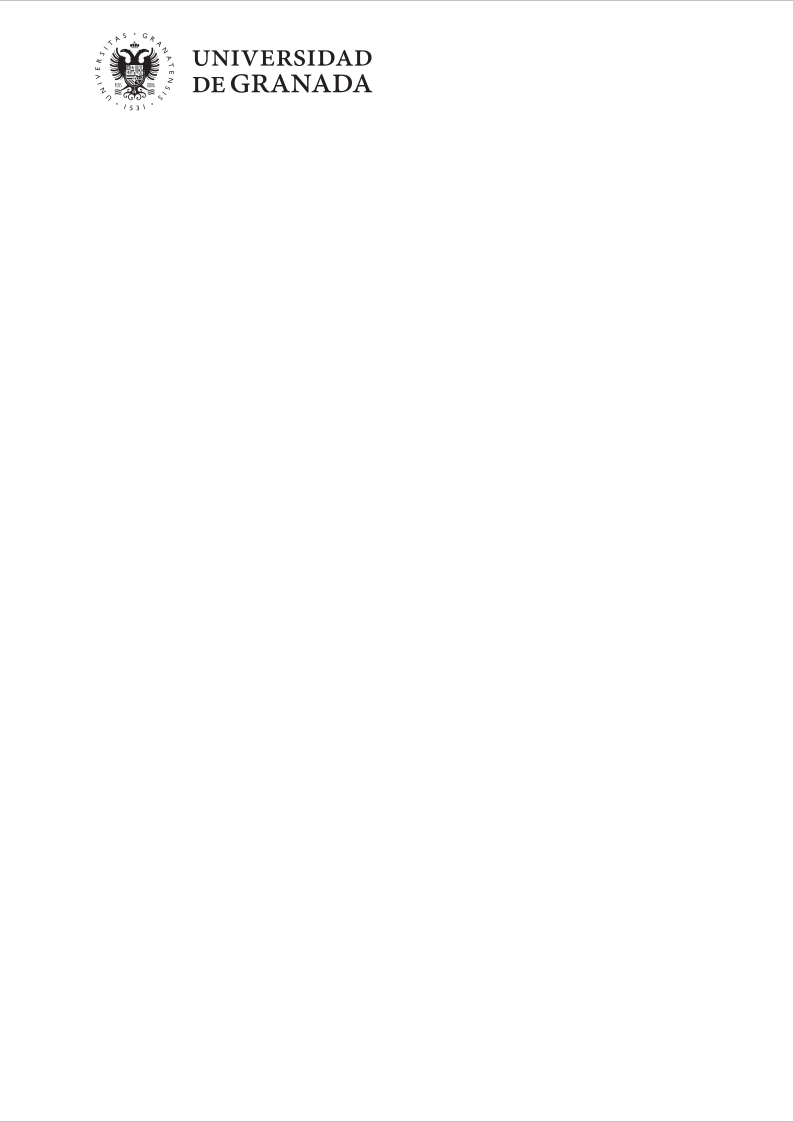
\includegraphics[width=\paperwidth,height=\paperheight,%
			keepaspectratio]{portada-ugr-sencilla}%
			\vfill
}}}

\usepackage{listings} % Para la inclusión de trozos de código

% CABECERAS
% ---------------------------------------------------------------------
% Si queremos modificar las cabeceras del documento podemos usar el paquete
% `scrlayer-scrpage` de KOMA-Script. Consultar la documentación al respecto.
% \usepackage[automark]{scrlayer-scrpage}

% VARIOS
% ---------------------------------------------------------------------

%\usepackage{showkeys}	% Muestra las etiquetas del documento. Útil para revisar las referencias cruzadas.

% ÍNDICE 
% ----------------------------------------------------------------------
% \index{} para añadir un elemento e 
% \index{main!sub} para añadir un elementos "sub" bajo la categoría "main".
% \index{termino|textbf} para dar formato al número de página (negrita).
% \index{termino|see{termino relacionado}} para crear una referencia cruzada

% Ejemplo: \index{espacio homogéneo}, \index{superficie!mínima}, \index{esfera|see{espacio homogéneo}}

% Para generar el índice hay que compilar el documento con MakeIndex. Generalmente los editores se encargan de ello automáticamente.
\usepackage{makeidx}
%\usepackage{showidx} % Muestra en el margen del documento las entradas añadidas al índice. Útil para revisar el documento. Si está activo el índice no se genera
\makeindex

% ---------------------------------------------------------------------
% COMANDOS Y ENTORNOS
% ---------------------------------------------------------------------
% Cargamos un archivo externo donde hemos incluido todos los comandos
% propios que vamos a usar en el documento.
% DEFINICIÓN DE COMANDOS Y ENTORNOS

% CONJUNTOS DE NÚMEROS

  \newcommand{\N}{\mathbb{N}}     % Naturales
  \newcommand{\R}{\mathbb{R}}     % Reales
  \newcommand{\Z}{\mathbb{Z}}     % Enteros
  \newcommand{\Q}{\mathbb{Q}}     % Racionales
  \newcommand{\C}{\mathbb{C}}     % Complejos

% TEOREMAS Y ENTORNOS ASOCIADOS

  % \newtheorem{theorem}{Theorem}[chapter]
  \newtheorem*{teorema*}{Teorema}
  \newtheorem{theorem}{Teorema}[chapter]
  \newtheorem{prop}{Proposición}[chapter]
  \newtheorem{lema}{Lema}[chapter]
  \newtheorem{corolario}{Corolario}[chapter]

    \theoremstyle{definition}
  \newtheorem{definicion}{Definición}[chapter]
  \newtheorem{ejemplo}{Ejemplo}[chapter]

    \theoremstyle{remark}
  \newtheorem{observacion}{Observación}[chapter]


% --------------------------------------------------------------------
% INFORMACIÓN DEL TFG Y EL AUTOR
% --------------------------------------------------------------------
\usepackage{xspace} % Para problemas de espaciado al definir comandos

\newcommand{\miTitulo}{Visualización realista por Monte-Carlo\xspace}
\newcommand{\miNombre}{Antonio Checa Molina\xspace}
\newcommand{\miGrado}{Grado en Ingeniería Informática y Matemáticas}
\newcommand{\miFacultad}{Facultad de Ciencias}
\newcommand{\miUniversidad}{Universidad de Granada}
% Añadir tantos tutores como sea necesario separando cada uno de ellos
% mediante el comando `\\\medskip` y una línea en blanco
\newcommand{\miTutor}{
  Carlos Ureña Almagro \\ \emph{Departamento de Lenguajes y Sistemas Informáticos} 
}
\newcommand{\miCurso}{2019-2020\xspace}

% HYPERREFERENCES
% --------------------------------------------------------------------
\usepackage[pagebackref]{hyperref}
% Opciones para el paquete hyperref
%----------------------------------

\hypersetup{%
  % hidelinks,            % Enlaces sin color ni borde. El borde no se imprime
  linkbordercolor=0.8 0 0,
  citebordercolor=0 0.8 0,
  citebordercolor=0 0.8 0,
  colorlinks = true,            % Color en texto de los enlaces. Comentar esta línea o cambiar `true` por `false` para imprimir el documento.
  linkcolor = [rgb]{0.5, 0, 0}, % Color de los enlaces internos
  urlcolor = [rgb]{0, 0, 0.5},  % Color de los hipervínculos
  citecolor = [rgb]{0, 0.5, 0}, % Color de las referencias bibliográficas
	pdftitle={\miTitulo},%
	pdfauthor={\textcopyright\ \miNombre, \miFacultad, \miUniversidad},%
  pdfsubject={Trabajo de fin de Grado},%
	pdfkeywords={},%
	pdfcreator={pdfLaTeX},%
}

% Redefinición del estilo para mostrar las referencias cruzadas en la bibliografía.
\renewcommand*{\backref}[1]{}
\renewcommand*{\backrefalt}[4]{{\footnotesize [%
    \ifcase #1 No citado%
    \or Citado en pág.~#2%
    \else Citado en págs. #2%
    \fi%
]}}

% Etiquetas en español para el comando \autoref
\def\chapterautorefname{Capítulo}
\def\appendixautorefname{Apéndice}
\def\sectionautorefname{Sección}
\def\subsectionautorefname{Subsección}
\def\figureautorefname{Fig.}
\def\tableautorefname{Cuadro}

\def\teoremaautorefname{Teorema}
\def\proposicionautorefname{Proposición}
\def\lemaautorefname{Lema}
\def\corolarioautorefname{Corolario}
\def\definicionautorefname{Def.}
\def\observacionautorefname{Observación}
\def\ejemploautorefname{E.j.}

% Pone automáticamente un parántesis para las ecuaciones
\def\equationautorefname~#1\null{Ec.~(#1)\null}

\RequirePackage{amsmath}
\usepackage{amsthm}
%\usepackage[spanish]{babel}
\usepackage[utf8]{inputenc}
\usepackage[vmargin=2cm,hmargin=2cm]{geometry}
\usepackage{enumerate}
\usepackage{dsfont}
\usepackage{graphicx}
%\usepackage[usenames]{color}
%\usepackage[dvipsnames]{xcolor}
%\usepackage{accents}
\usepackage[many]{tcolorbox}
\usepackage{upgreek}
\usepackage{import}
\usepackage{xifthen}
\usepackage{pdfpages}
\usepackage{transparent}

\newcommand{\incfig}[1]{%
	\def\svgwidth{0.5\columnwidth}
	\import{./figures/}{#1.pdf_tex}
}


\newtheorem{mydef}{Definición}
\newtheorem{mycorolario}{Corolario}
%\newtheorem{theorem}{Teorema}
%\newtheorem{prop}{Proposición}
%\newtheorem{lema}{Lema}
\newtcolorbox{myboxRed}{colback=red!5!white,colframe=red!75!black}
\newtcolorbox{myboxBlue}{colback=blue!5!white,colframe=blue!75!black}
\newtcolorbox{myboxPrinciples}[2][]{colback=green!10!white,colframe=green!65!black, title={#2}, #1}
\begin{document}

% --------------------------------------------------------------------
% FRONTMATTER
% -------------------------------------------------------------------
\frontmatter % Desactiva la numeración de capítulos y usa numeración romana para las páginas

% \pagestyle{plain} % No imprime cabeceras

% !TeX root = ../libro.tex
% !TeX encoding = utf8

%*******************************************************
% Titlepage
%*******************************************************
\begin{titlepage}
  \AddToShipoutPicture*{\BackgroundPic}
  \phantomsection 
  \pdfbookmark[1]{Título}{title}

  % Para que el título esté centrado en la página.
  % Los valores numéricos deberán elegirse de acuerdo con el diseño de
  % página (sobre todo si se cambia la opción BCOR o DIV).
  \begin{addmargin}[2.575cm]{0cm}
  \begin{flushleft}
    \Large  
    \hfill\vfil

    \textsf{\miFacultad}
    \vfill\vfill

    {\huge\textsf\miGrado} \vfill


    \textsc{Trabajo fin de grado}

    \begingroup
    \Huge{\miTitulo} \\ \bigskip
    \endgroup

    \vfill\vfill\vfill\vfill

    \textsf{\normalsize{Presentado por:}}\\
    {\Large\textrm{\miNombre}}

    \vfill
    \textsf{Curso académico \miCurso}
  \end{flushleft}  
  \end{addmargin}       

\end{titlepage}   
\cleardoublepage
\endinput
                    
% !TeX root = ../libro.tex
% !TeX encoding = utf8

%*******************************************************
% Little Dirty Titlepage
%*******************************************************

\thispagestyle{empty}

\begin{center}
  \large  

  \vspace*{\stretch{1}}

  \begingroup
  \huge{\miTitulo} \\ \bigskip
  \endgroup

  \textrm{\miNombre}

  \vspace{\stretch{5}}

\end{center}  

\newpage
\thispagestyle{empty}

\hfill

\vfill

\noindent\miNombre \textit{\miTitulo}.

Trabajo fin de grado. Curso académico \miCurso.

\begin{minipage}[t]{0.25\textwidth}
  \flushleft
  \textbf{Director}
\end{minipage}
\begin{minipage}[t]{0.45\textwidth}
  \flushleft
  \miTutor
\end{minipage}
\begin{minipage}[t]{0.30\textwidth}
  \flushright
  \miGrado
  \medskip

  \miFacultad
  \medskip

  \miUniversidad
\end{minipage}
\begin{flushleft}
\end{flushleft}

\endinput
                     
\include{preliminares/declaracion-originalidad}   
% !TeX root = ../libro.tex
                % Opcional
% !TeX root = ../libro.tex
% !TeX encoding = utf8

%*******************************************************
% Table of Contents
%*******************************************************
\phantomsection
\pdfbookmark[0]{\contentsname}{toc}

\setcounter{tocdepth}{2} % <-- 2 includes up to subsections in the ToC
\setcounter{secnumdepth}{3} % <-- 3 numbers up to subsubsections

% \manualmark
% \markboth{\textsc{\contentsname}}{\textsc{\contentsname}}
\tableofcontents 

%*******************************************************
% List of Figures and of the Tables
%*******************************************************

    % *******************************************************
    %  List of Figures
    % *******************************************************    
    %\phantomsection 
    %\listoffigures

    %*******************************************************
    % List of Tables
    %*******************************************************
    %\phantomsection 
    %\listoftables
    
    %*******************************************************
    % List of Listings
    % The package \usepackage{listings} is needed
    %*******************************************************      
	  % \phantomsection 
    % \renewcommand{\lstlistlistingname}{Listados de código}
    % \lstlistoflistings 

\cleardoublepage
            
\include{preliminares/agradecimientos}            % Opcional

% \pagestyle{scrheadings} % A partir de ahora sí imprime cabeceras

\include{preliminares/summary}                    
\include{preliminares/introduccion}               

% --------------------------------------------------------------------
% MAINMATTER
% --------------------------------------------------------------------
\mainmatter % activa la numeración de capítulos, resetea la numeración de las páginas y usa números arábigos

\setpartpreamble[c][0.75\linewidth]{%
	\bigskip % Deja un espacio vertical en la parte superior
}

% Añadir tantos capítulos como sea necesario
%\tableofcontents

\newpage



\chapter{Introducción}
%Hablar de la gente que referencia el paper de 2013 como motivación, de conseguir reducir varianza y tiempo de ejecución
En los últimos años ha habido un auge de exigencia en fotorrealismo desde varios ámbitos. En la industria del cine se ha usado en animaciones y efectos especiales, sin irnos más lejos en 2019 se ha estrenado una nueva versión de \textit{El rey león}, teniendo como uno de sus objetivos obtener un efecto de imagen real de la antigua película animada. La mayoría de catálogos de interiorismo utilizan técnicas fotorrealistas para que los clientes puedan visualizar los muebles con mayor facilidad, al igual que los arquitectos a la hora de vender un proyecto. Incluso si buscamos técnicas concretas como ray-tracing, veremos noticias de principio de año de NVIDIA, que utilizó este término en su conferencia CES 2019 (\cite{nvidia}), con el fin de hablar de sus últimos avances. 

Estas exigencias provienen de un avance de la tecnología, que se ha sustentado principalmente en la mejora de dispositivos gráficos, permitiendo mayor velocidad de cálculos, y en los estudios de técnicas de renderización. Sin embargo, los costes de producción también se han incrementado, tanto en tiempo como en dinero. Si el mercado sigue expandiéndose hacia otros ámbitos, como por ejemplo los recientes proyectos de museos virtuales, es de esperar que cada paso hacia algoritmos más rápidos y eficaces suponga una disminución de costes a escala global en cada una de las aplicaciones mencionadas. De esta forma, el estudio de la visualización fotorrealista cumple dos objetivos fundamentales: resuelve un problema real del cual dependen numerosos proyectos y abarata los costes de producción de estos. 

Si bien hay numerosas técnicas utilizadas, en particular ray casting o rasterización, en este trabajo nos centraremos en técnicas basadas en trazado de rayos (ray-tracing), como distirbuted ray-tracing o path-tracing. El algoritmo ray-tracing, propuesto por Turned Whitted en 1980 en \cite{Whitted} y simple de entender, es una de las mejores técnicas para producir efectos de iluminación global, como múltiples reflejos y sombras, en la creación de imágenes. Su principal problema es el tiempo de cómputo necesario, por lo que todos los métodos enfocados a reducirlo son de especial relevancia. Hasta el año 2000 se pensaba que estos algoritmos nunca serían competitivos frente a los basados en métodos de elementos finitos, pero a partir de entonces el avance tanto en hardware como en optimización del procedimiento permitió demostrar que esto no era cierto. Hoy en día son estos algoritmos basados en path-tracing los que dominan la elaboración de imágenes digitales.

En este trabajo estudiaremos este algoritmo y su estrecha relación con la ecuación de renderización, o \textit{rendering equation}. Esta ecuación fue introducida por primera vez en \cite{kajiya}, donde se veía cómo se podía resolver mediante muestreo aleatorio de trayectorias con el punto origen del observador de la imagen que se crea. Cada rayo producido por ray-tracing necesita hallar la radiancia que viaja a lo largo del rayo, para poder producir los colores de los píxeles en la imagen final. Esta radiancia depende de forma directa de las luces que se encuentran en la escena. Nuestro objetivo final es muestrear fuentes de luz de forma directa, técnica introducida por primera vez en \cite{cook}, observar los métodos diferentes que hay para realizar esto y compararlos. Para ello, es necesario hacer uso de técnicas creadas en la última década. En particular, varias referencias principales para esto han sido \cite{ur2013}, \cite{ur2017} y \cite{ur2018}. En total con las fuentes hay tres tipos de luces de área que considerábamos estudiar: rectángulos, que son los más comunes en escenas de renderización, discos y proyecciones de casquetes esféricos. 

Toda la información recopilada aquí es ampliamente conocida y usada por varios motores de renderización. Se puede observar el software Arnold (\cite{arnold}), creado por la compañía Solid Angle, como ejemplo de uso actual de este tipo de técnicas de muestreo. También son recomendadas en otras investigaciones, como en 
\cite{productionVolume}, debido a que funcionan mejor que las técnicas usuales.

La estructura del trabajo se divide en preliminares, donde se definen todos los conceptos necesarios sobre el algoritmo del ray-tracing, el muestreo de luces de área y los experimentos sobre las diferentes técnicas que probamos. Más concretamente, en los preliminares primero hablamos del algoritmo general y de su relación con la ecuación de renderización. Siendo esta última un problema de resolver una integral, se estudian las técnicas usuales a la hora de conseguir cálculos precisos y rápidos. Exploramos la integración con el método de Monte-Carlo junto a varios ejemplos de uso. De la misma forma, introducimos la estratificación con varios ejemplos para que se vea el efecto en los cálculos finales. También explicamos el concepto de muestreo por importancia, o \textit{importance sampling}, y por qué es especialmente relevante en este trabajo. Mencionamos el rechazo de muestras como técnica necesaria en algunos procedimientos. Por último, estudiamos la implementación utilizada en el trabajo, basada en el trabajo de Peter Shirley en \cite{Weekend} y sus obras posteriores, \cite{NextWeek} y \cite{RestOfYourLife}. El código adjuntado es en su mayoría proveniente de esta fuente, siendo solo tres archivos aparte necesarios para este trabajo en particular. 

Los principales objetivos de este trabajo eran:
\begin{itemize}
	\item Introducir el algoritmo de ray-tracing y trabajar con su implementación.
	\item Estudiar las técnicas de muestreo por área e introducirlas en la implementación del ray-tracing.
	\item Estudiar las técnicas de muestreo por ángulo sólido con las investigaciones de \cite{ur2013}, \cite{ur2017} y \cite{ur2018}. Hacer un estudio comparativo con otras técnicas e implementarlas.
\end{itemize}

Se han conseguido todos los objetivos salvo la implementación de proyecciones de casquetes esféricos, basada en \cite{ur2018}, la cual queda como posible continuación en el futuro.

\section{Resumen}
En este trabajo estudiamos el muestreo directo de luces de área como herramienta para acelerar el proceso de renderización mediante ray-tracing, con menos error usando el mismo número de muestras.

Usando una implementación base del algoritmo, se han añadido las clases y código necesario para poder hacer muestreo directo de luces mediante dos métodos: por área y ángulo sólido. En la memoria se han introducido los conceptos necesarios para entender todo el código, en relación al ray-tracing. Es de especial relevancia la sección de la ecuación de renderización y el muestreo por importancia.

Este estudio se ha dividido según la forma de la fuente de luz. Se han realizado con luces rectangulares y con discos. La construcción del muestreo por área se ha realizado de forma usual, por no ser un algoritmo complicado, y la del ángulo sólido se ha hecho en base a las fuentes referenciadas.

Se han realizado experimentos midiendo el tiempo y el error de ambos métodos, viendo cómo afecta el tamaño de la luz a los resultados. Este estudio también se realiza en función del número de muestras por píxel creadas. Hemos comprobado si las hipótesis que deducíamos en la teoría se mantienen en la práctica.

Se adjunta con este trabajo el código realizado para obtener los resultados y las gráficas. Si bien el código base no está documentado, debido a que no es código nuestro, se han comentado los archivos nuevos de forma que sean fáciles de entender habiendo leído la memoria.

Palabras clave: integración por Monte-Carlo, iluminación global, path-tracing, luces de área, ángulo sólido.

\section{Extended summary}
In this document we try to introduce the basic definitions and concepts to easily understand the algorithm of ray tracing, studying how to apply importance sampling to sample area lights and doing experiments with different methods. All this can be understood by any student who has knowledge about probability, integration and linear algebra.

The reader may notice that we've only applied this techniques to particular examples of area lights. We've tried to add references that talk about other kind of lights, and how to sample them with solid angle. As they're relatively new and work better than previous works, there is still an interest in studying this algorithms.

Because of each section having its own details and concepts, we'going to summarize each in the following paragraphs.

It's important to note that this ray tracing algorithm has some differences with the original one. We try to explain some of them. One example could be the soft shadows, obtained by simulating a lot of rays, and not sampling directly to the light every point. 

\textbf{Chapter 1, introduction}: We introduce the current context and the relevance of photorealism in different industries: cinema, videogames or interior design. This works as a justification of why studying ray tracing is important. We summarize the structure of the entire document and the goals of it. It's important to clarify that not all of the goals were met, we leave this for further work. We also include the usual summary and the extended one.

\textbf{Chapter 2, ray tracing}: We define and explore the algorithm of ray tracing. This is the foundation of the rest of the document, that's why it's the largest chapter. First we define the algorithm itself, and the differences and similarities between this process and taking a picture with a camera in real life. After that, we divide the implementation in different objects: cameras, rays, the scene itself, scaterring and refraction effects, sampling lights (and the difference between point lights and area ones), shadows, indirect lightning and ray propagation. We talk about how, essentially, the algorithm is constructing rays and calculating the radiance that ray obtains from the scene. That's when we introduce the rendering equation, that formalizes this problem and it gives us an integration problem.

We also introduce the rendering equation. This lets us justify some parts of the ray-tracing implemented here, which can produce soft shadows, that usually ray tracer can't do. We make an analogy between the rendering equation, that would mean the perfect photorealism, with the calculations made in our implementation. However, it's important to note that this is no path tracing, and that there are differences between what that and our ray tracing algorithm.

After we've introduced the rendering equation, we focus on methods to easily calculate the integral previously mentioned. We explore the most popular ones. The most basic one, and the one that gives the title to this document, is Monte Carlo integration. With it, we try to approximate the solution with discrete sums over some samples. We make the connection of this method with the law of large numbers, that justifies why it works. We obtain the expected error, which depends on the number of samples, so with more samples less expected error. As this is a fundamental concept, we try to clarify it further with a particular example, trying to approximate the area of a quarter of a circle.

Another important concept to decrease error is stratification. We establish the formal definition of it, why it works and we also apply it to the previous example. We make two different experiments with different numbers of stratification subsets, to see how this affect the results. We conclude that this lets us decrease the error while having the same number of sample rays.

The next technique we talk about is importance sampling. By sampling with a probability density function similar to the one we're integrating, we decrease the errors of the approximation. We explore the origins of the method, its efficiency and its problems. In general, it's true that we can take advantage of this fact, but it's usually hard to find any function similar to the one we're integrating. We add an example of this too, so we can see it working, which ends up with the exact result in the first samples, and failing, where the errors are similar to the original uniform distribution, sometimes even worse. We conclude that it's difficult to use but powerful.

We also introduce the term of rejection sampling. This technique is based on the fact that if we have a set $A$ and a subset of it, $B$, we can sample the second one with a distribution of the first. We reject or ignore any sample outside of the subset we're studying. As we explain here, it's a simple algorithm that lets us work with complex scenarios, but it increases the time needed to sample, because we're wasting a part of our samples that don't affect the calculation at all. While it's best to avoid if possible, we talk about the parts of ray tracing where we have to do this: shadows and sampling only the entire sphere of directions, instead of the hemisphere.

Finally, we introduce the source code of the implementation of the experiments, that will lets us change parts of the ray tracing algorithm. It's important to note that not every part explained on this chapter is included in the implementation. Some exceptions include ray propagation and stratification, but this doesn't affect much the experiments made. We summarize the properties the code has, the structure of it and the names of the files that contains each object. We include an example made with this implementation, with the four basic materials added to it: lambertian, metal, dielectric and emission. We also included a flowchart of the main process, to clarify how the main part of the ray tracing algorithm works. 

\textbf{Chapter 3, area lights and direct light sampling}: After we've introduced all the basic concepts of ray tracing, we start to talk about the particular topic of this document, which is direct area light sampling. We justify direct light sampling as applying importance sampling to the rendering equation, because lights are the part of the scene with most emission (the rest is just indirect lightning due to refractions and scattering). We also introduce the concept of mixture probablity density functions, that will lets us apply direct light sampling without losing the indirect parts. 

Furthermore, we explore the differences between two sampling methods, area and solid angle sampling. If we sample based on the area, we just take an uniform distribution over the light, take a point and generate a ray towards it. However, this doesn't generate an uniform distribution over the subset of the hemisphere of directions, the one that actually define the space for our rays. This way, if we want to sample with this property we need solid angle sampling, so there is uniform sampling over the hemisphere of directions. We add a figure explaining how this two sampling work, with their projected points on the sphere, so it's clear the problem of the area sampling. There we can see the clusters of points near the extreme of the projection of the lights.


In general, we explain that it's far more difficult to sample with solid angle because it depends on the shape of the area. For some particular examples we can calculate it, and that's what we do in the next chapter.

\textbf{Chapter 4, experiments}: In this chapter we explore two particular area lights with both area and solid angle sampling: rectangles and disks. For rectangles, it's easy to generate an uniform distribution over them for area sampling, given an uniform distribution over an open interval in the real line. We implement solid angle sampling using an algorithm created by experts on the field, who created an area-preserving parametrization from the unit square to the projected rectangle on the sphere. This lets us generate random samples on the projected rectangle with all the desired properties, in particular, we apply this with an uniform distribution. We compare and analyze the results.

It's also easy to generate an uniform distribution over a disk to generate area sampling, using polar coordinates and the square root, and really hard to do solid angle sampling. For that we also apply a relatively new algorithm, that the reader can see in the references. It's important to note that here we must apply root finding and integration algorithms. While we apply some methods (in particular, bisection and Simpson's rule), we try to explore the differences between this implementation and the one recommended in the references. After that, we analyze and compare the results again.

\textbf{Chapter 5, conclusion}: We summarize the results and we try to establish the ground for further work. One example of this could be the projected spherical caps, with a solid angle sampling method created recently. This algorithm was not implemented here because of lack of time. It could be interesting to see the relationship between this work and the other two explained here.

Keywords: Monte-Carlo integration, global illumination, path-tracing, area lights, solid angle.


\chapter{Preliminares: teoría de ray-tracing y muestreo}
En este capítulo nos dedicaremos a presentar la teoría que sustenta el algoritmo del ray-tracing. Debido a que nuestro trabajo consiste en estudiar un apartado particular de este algoritmo, el de muestreo directo de luces y los diferentes métodos para realizarlo, es fundamental conocer dónde se sitúa en el procedimiento general.

Se han intentado exponer de la forma más sencilla posible, dándole más importancia a que el lector entienda las ideas detrás de los conceptos antes que a una formalización exacta del algoritmo. Esto se debe a dos motivos: facilita la comprensión de los apartados posteriores, que no necesitan de los detalles exactos de la construcción del ray-tracing; el código junto a las referencias presentadas es más que suficiente detalle para entender todo lo que se explica a continuación. 

Por esto mismo, los conocimientos previos necesarios para entender este apartado y el resto de secciones son definiciones básicas de álgebra lineal, integraciones y distribuciones de probabilidad. Como veremos, el proceso de renderización está estrechamente conectado a  resolver un problema de integración. Por esto mismo, exploraremos los métodos básicos usados para resolver este problema: Monte-Carlo, estratificación y rechazo de muestras. Por último hablaremos de la implementación usada, creada en su mayoría por el trabajo de Peter Shirley en \cite{Weekend} y \cite{NextWeek}.

\section{Algoritmos basados en Path-tracing}
Dentro de la renderización fotorrealista, el objetivo es conseguir una imagen que sea lo más parecida a una fotografía de los objetos que estamos modelando. Si bien hay varios algoritmos que consiguen un efecto parecido, el más popular entre ellos es el algoritmo del ray-tracing, propuesto por Turner Whitted en \cite{Whitted}. Este fue uno de los comienzos  del uso de técnicas de renderización con capacidad de producir resultados realistas con iluminación global. En esta sección exploraremos qué necesita este procedimiento, que usaremos como base para el resto del trabajo.

La esencia del ray-tracing es considerablemente simple, ya que se basa solo en seguir el camino de un rayo de luz, atravesando la escena que queremos renderizar, y partiendo desde nuestro punto de vista. El rayo interactúa con las superficies que interseca, rebotando entre los diferentes objetos, guardando finalmente un valor asociado al color producido por dichos objetos. En la figura \ref{fig:raytracing} se puede ver un esquema de un par de rayos en una escena sencilla con una sola luz y un solo objeto. Cuando los rayos no son capaces de llegar a una fuente de luz desde un punto, sin intersecar con un objeto en medio, se generan sombras. El paralelogramo es la imagen que se genera, donde cada píxel recibe color de los rayos que lo traspasan.

\begin{figure}[ht]
	\centering
	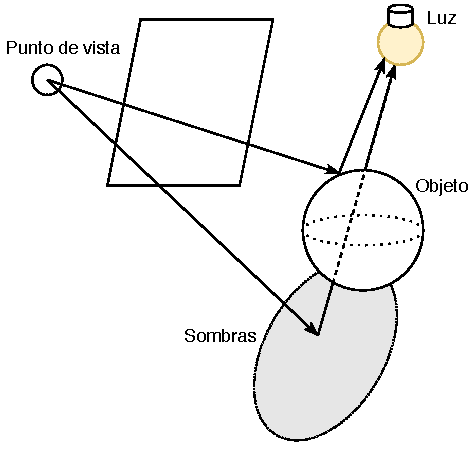
\includegraphics[width=0.6\textwidth]{raytracing}
	\caption{Ejemplo sencillo de rayos de ray-tracing partiendo desde un punto de vista, un paralelogramo que representa la imagen que se está produciendo, un objeto de la escena en el que rebota uno de los rayos y una luz.}
	\label{fig:raytracing}
\end{figure}

Hay una diferencia crítica en cómo funcionan las luces reales con cómo las simulamos en el algoritmo. Normalmente, son los rayos de luz los que van desde las luces hasta los objetos, y luego llegan a nuestros ojos, donde los nervios ópticos transforman lo que reciben en impulsos que nuestro cerebro reconoce como colores e intensidades. Es decir, los rayos no parten de los ojos, así que uno podría plantearse por qué en el algoritmo se hace de esta manera. La respuesta recae en que la mayoría de rayos de luz no generan ningún tipo de imagen en nuestros ojos, si no que rebotan entre los objetos sin llegar a tocarnos. Debido a que nuestro objetivo es únicamente producir la imagen desde un punto de vista concreto, nos interesan solo los rayos que vayan a intersecar en el marco de la imagen, por lo que partir desde el propio ojo es la forma natural de asegurarnos esto.

El algoritmo en sí necesita simular varios elementos. Vamos a resumirlos, basándonos en la separación hecha en \cite[Chapter~1]{pbrt}:
\begin{itemize}
	\item \textbf{Cámaras}: En este caso con una cámara querremos modelar cómo se ve la escena, y qué propiedades tendrá la imagen final. Como ejemplo, en la figura \ref{fig:raytracing} la cámara sería el punto de vista, u ojo, junto al paralelogramo que representa el film donde se guardan los colores percibidos desde la escena. Existen numerosos tipos de cámaras, pero la más básica de todas se puede modelar solo con un punto de vista origen y un rectángulo, junto al número de píxeles que querremos ver en la imagen final, tanto a lo ancho como a lo alto. Por cada píxel crearemos varios rayos que lo atraviesen, y el color final del píxel será una media de los valores recibidos, de forma similar a como lo haría una cámara real. En este trabajo nos quedaremos con este tipo de cámaras sencillas.
	\item \textbf{Intersección de rayo-objetos}: Una vez decididos los rayos que se generan desde el ojo hacia el marco de la imagen, necesitamos saber en qué objetos de la escena intersecan, y en qué punto de estos. No solo eso, si no que necesitaremos también ciertas propiedades del punto en cuestión, como el normal del objeto en ese punto. Ciertos ray-tracers más complejos requieren aún más información geométrica del punto, como el que se crea en \cite{pbrt}, pero en nuestro trabajo el normal será suficiente. Otro tema interesante sobre la intersección del rayo con los objetos es cómo calcularla de forma eficiente. Los detalles sobre cómo se puede realizar de forma simple, y cómo se ha hecho en este trabajo, están contenidos en la sección \ref{Implementacion}.
	\item \textbf{Dispersión de la luz}: Una vez que tenemos un punto de intersección del rayo con un objeto de la escena, nuestro objetivo es saber cuánta radiancia vuelve desde este punto hacia la cámara. En el cálculo hará falta saber las propiedades del propio objeto que intersecamos, provocando al menos uno de los siguientes efectos: absorción, causando que el rayo pierda parte de su intensidad; reflexión, generando un nuevo rayo en una nueva dirección y recibiendo la radiancia que se genera con él; y refracción, cuando la superficie es transparente o translúcida y parte del rayo entra dentro del objeto en una dirección diferente a la original. Esta información se suele modelar en el propio objeto.
	\item \textbf{Luces}: Por otro lado, no todas las luces funcionan de la misma forma. Una luz de un solo punto funciona esencialmente diferente a una luz de área, que está asociada a un objeto de la propia escena con la propiedad de emisor. Esto es importante remarcarlo, debido a que este trabajo se dedica concretamente a una mejora de muestreo de luces de área particulares. El programa debe ser capaz de modelar distintos tipos de luces, según la complejidad de la escena que queramos crear.
	\item \textbf{Visibilidad}: Cuando, dado un punto en una superficie, ninguna luz es visible desde él (es decir, todos los rayos entre ese punto y las luces intersecan con un objeto opaco en su camino), se producen sombras, tal y como se ejemplifica en la figura \ref{fig:raytracing}. Si no hay ningún objeto, entonces hay visibilidad entre el punto y la luz y esta última contribuye al valor final del propio rayo. 
	
	\item \textbf{Luces indirectas}: Tal y como hemos mencionado anteriormente, es posible que los rayos tengan que generar rayos reflejados y refractados, con direcciones diferentes a la del original, y observar qué luz reciben. Este procedimiento es el que estábamos aplicando, por lo que el algoritmo es recursivo, y es precisamente esto lo que permite hallar las luces indirectas con más facilidad que otros algoritmos de renderización. 
	
	\item \textbf{Propagación de los rayos}: La presencia de medios participativos, como la niebla o el humo, son capaces de distorsionar una imagen debido a que afectan a los rayos que los atraviesan. Si bien esto es importante en el algoritmo en general, a lo largo de este trabajo no simularemos medios participativos.
\end{itemize}

A continuación, vamos a explicar la parte más específica del ray-tracing que vamos a explorar en este trabajo. La ecuación de renderización, que se utiliza en el paso de dispersión de la luz, cuyo objetivo es calcular, mediante una ecuación integral, la radiancia que llega a un punto dado del espacio. Es necesario entender que resolver esta ecuación es lo más costoso a la hora de la renderización realista.

\section{Ecuación de renderización}
\label{rendering}
La ecuación de renderización, o ecuación del transporte de la luz, describe la distribución de la radiancia. Esta ecuación es fundamental de cara a establecer cualquier algoritmo de trazado de rayos, ya que contiene los cálculos necesarios para una precisa iluminación de la escena. Su complejidad se basa en que contiene todos los datos que podrían afectar a la radiancia de un punto, como puede ser el color de un punto cercano en la escena. 

Antes de explicar la ecuación de renderización necesitamos saber cómo funciona la reflectancia de la radiación contenida en los rayos. Más formalmente, dado un punto $p$ y una dirección $\omega_o$, que representa desde dónde vemos el punto, queremos saber cuánta radiación se refleja desde la dirección $\omega_i$, que llamaremos $L_i(p, \omega_i)$. A esta función se le llama BRDF, proveniente de \textit{bidirectional reflectance distribution function}, o función de distribución de reflectancia bidireccional en español, y se nota como $f_r(p, \omega_o, \omega_i)$. 

Esta función cumple tres propiedades importantes: es positiva, tiene reciprocidad, $f_r(p, \omega_o, \omega_i) = f_r(p, \omega_i, \omega_o)$, y conserva la energía:
$$\int_{\Omega } f_r(p, \omega_o, \omega_i) \cos(\phi_i) d\omega_i \leq 1,$$
donde $\Omega$ denota la semiesfera de direcciones alrededor del normal de la superficie en el punto $p$.

Por otro lado también tenemos la función de distribución de transmitancia bidireccional (BTDF), que describe la radiancia transmitida, es decir, que traspasa el material hacia el otro lado de la superficie. Hay que notar que no existen dos ángulos para los que tenga sentido definir ambas funciones, ya que una trabaja solo en un lado de la superficie y otra trabaja en el contrario. Se puede definir de una forma similar a la BRDF, y se suelen escribir juntas como la BSDF, o función de distribución de difusión bidireccional. Esta función se nota como $f(p, \omega_o, \omega_i)$ y recordemos que es simplemente unir las dos funciones anteriores, ya que ambas no estaban definidas en los mismos dominios. Por lo que $f$ nos proporciona la radiancia reflejada desde la parte de la superficie donde se encuentra el punto de vista y la transmitida del contrario. De esta forma, si queremos medir la radiancia hacia $\omega_o$ global solo tenemos que calcular la siguiente integral:
$$ \int_{S^2} f(p, \omega_o, \omega_i) L_i(p, \omega_i) |\cos(\phi_i)| d\omega_i.$$

Volviendo a la ecuación de renderización, la clave de la ecuación es el equilibrio de la energía. Esto implica que la energía que proviene de un punto $p$ con dirección $\omega_o$ debe ser igual a la emitida por el material en el que se encuentra el punto, $L_e$, sumada a la radiancia dispersada, que es la integral anterior. Juntando esto tenemos:
$$L_o(p, \omega_o) = L_e(p, \omega_o) + \int_{S^2} f(p, \omega_o, \omega_i) L_i(p, \omega_i) |\cos(\phi_i)| d\omega_i,$$
donde hemos denominado a la radiancia obtenida desde $p$ con dirección $\omega_o$ la función $L_o$. Aunque esta sea la ecuación general con las dos funciones, de reflectancia y de transmitancia, juntas, es también interesante ver cómo queda si nos fijamos solo en la radiancia reflejada en un punto de una superficie. Es decir, utilizar $f_r$ en lugar de $f$. Se puede ver como un caso particular de la anterior ecuación, y nos quedaría:
$$L_o(p, \omega_o) = L_e(p, \omega_o) + \int_{\Omega} f_r(p, \omega_o, \omega_i) L_i(p, \omega_i) |\cos(\phi_i)| d\omega_i,$$
donde es importante notar el cambio de dominio de la integral, donde vuelve a ser $\Omega$ en lugar de todas las posibles direcciones.

Volviendo con la ecuación de renderización en su forma más general, si asumimos que no existe propagación de rayos ni medios participativos, se tiene que la radiancia incidente en $p$ con dirección $\omega$ es igual a la que proviene de un punto $t_{p,\omega}$ con dirección $-\omega$, siendo $t_{p,\omega}$ el primer punto de intersección del rayo $p+\lambda \omega$ con la escena. En el caso de que no haya punto de intersección, definimos la radiancia proveniente de ese punto como $0$. Si sustituimos en la ecuación anterior, obtenemos:
$$L_o(p, \omega_o) = L_e(p, \omega_o) + \int_{S^2} f(p, \omega_o, \omega_i) L_i(t_{p,\omega_i}, -\omega_i) |\cos(\phi_i)| d\omega_i,$$
que tiene el principal problema de que es una definición recursiva.

Cuando hablamos de un método consigue resultados fotorrealistas es porque aproxima bien la ecuación de renderización. En la implementación concreta de ray-tracing usada en este trabajo, la esencia de lo que estamos haciendo es enviar rayos desde la cámara, intersecar objetos, ver si emiten radiación y si no, continuar enviando rayos desde este punto final. Es decir, la base de la naturaleza recursiva del algoritmo es principalmente intentar aproximar los valores de radiancia de un punto en función de todos los contenidos en la semiesfera. Si estuviéramos aproximando solo esta ecuación y basando nuestro programa en ella, lo que tendríamos sería más bien un path tracing. En este caso, tenemos un número máximo de llamadas recursivas, de puntos en los que reflectar, y cuando llegamos a ese tope devolvemos el valor dado. 

De alguna forma, tanto las llamadas recursivas como la naturaleza de la integral ayudan a ver por qué en el ray tracing basado en los trabajos de Peter Shirley se suman los valores correspondientes a distintos rayos. Todo esto permite simular sombras y partes de iluminación global que con el algoritmo de ray tracing original (que solo envía un rayo que siempre se muestrea de forma directa con las luces) no se tenían.

De hecho, en el muestreo directo de luces también debemos hallar la integral de la radiancia obtenida por esa luz en nuestro punto. Debido a esto, nos interesará estudiar métodos para aproximar integrales, que veremos en las siguientes secciones.
\section{Integración por Monte-Carlo}
Las siguientes secciones en relación a la integración por Monte-Carlo, junto a la sección \ref{estratif} y \ref{rechazo} son fundamentales a la hora de entender por qué los algoritmos que exponemos en el trabajo funcionan mejor que los más naturales y simples. Estas secciones están basadas en las notas de \cite{RestOfYourLife}.

El método de Monte-Carlo es un procedimiento no determinista que tiene el objetivo de aproximar valores numéricos mediante muestreo aleatorio. Normalmente, se utiliza cuando encontrar el valor exacto es demasiado costoso. La integración de Monte-Carlo es cuando se aplica este método para resolver una integral. Esta integración es necesaria cuando no podemos encontrar una primitiva del integrando en cuestión, como es el caso en iluminación global. Carecemos de expresión analítica del integrando o de la primitiva, por lo que es obligatorio el uso de aproximaciones numéricas. Las alternativas a este método son el método de elementos finitos o las reglas de cuadratura multidimensionales, ambos integrando una función que intenta asemejarse a la que queremos integrar, pero estos la complejidad de estas alternativas aumenta exponencialmente con el número de dimensiones. La ventaja de Monte-Carlo es su eficiencia en problemas con multiples dimensiones, como es el caso de iluminación global. 

En general, el problema que resuelven estos métodos es el de aproximar $I = \int_{A}f(x) dx$, donde $A\subset\mathds{R}^n$ es el conjunto en el que queremos integrar la función $f:A\rightarrow\mathds{R}$. Veamos cómo funciona en concreto el método de Monte-Carlo. Siendo $\lambda(A)$ el volumen de dicho conjunto, sabemos que si $x_1, \hdots, x_m$ son puntos obtenidos de una distribución uniforme en $A$, entonces por la ley de los grandes números tenemos que:
$$\lim\limits_{m\rightarrow\infty} \lambda(A) \frac{1}{m} \sum_{i=1}^{m} f(x_i) = I.$$
Veamos esto con un caso concreto. Sea $n=1$, $A = [0,1]$ y $f(x) = \sqrt{1-x^2}$. La integral, que es igual al área bajo la curva, es un cuarto de un círculo de radio 1 y centro el origen. En este caso, $I = \pi/4$. Vamos a usar el método para aproximar este valor. Es importante notar que no hay posibilidad de acotar el error del valor aproximado, pero sí cómo varía el error asintóticamente frente al número de muestras, en función de $\frac{1}{\sqrt{N}}$, tal y como se menciona en \cite{Press}.

En la figura \ref{fig:montEx} podemos ver una gráfica del error conforme avanzamos el número de muestras, junto a la función $\frac{1}{\sqrt{N}}$. Se ha realizado un experimento independiente por cada $N$ posible, y se ha calculado la diferencia del valor estimado con $\pi/4$. Se pueden notar varias cosas con este sencillo ejemplo. Estamos en solo una dimensión, por lo que el muestreo es más efectivo, debido a que en varias dimensiones los puntos tienden a estar más alejados entre sí lo que produce más error final. Aun así, el error final que es de $0.002$, quizás para algo tan simple como una integral, sigue estando en el orden de las milésimas. Lo bueno es que el método es muy simple, y permite bastantes mejoras. Vamos a explorarlas en las siguientes secciones.


\begin{figure}[ht]
	\centering
	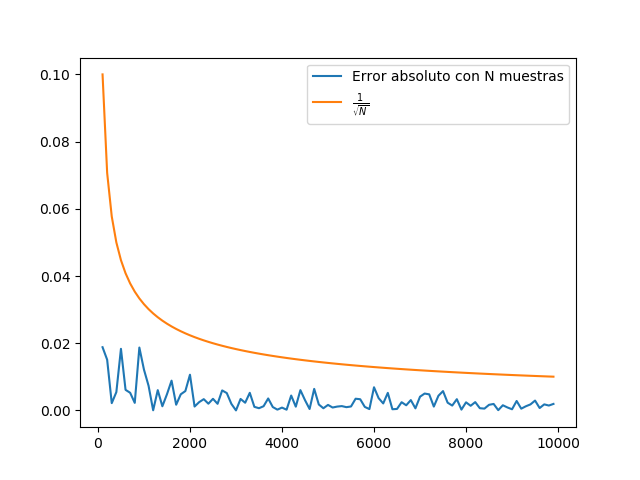
\includegraphics[width=0.6\textwidth]{error_mc_normal2}
	\caption{Errores absolutos en el ejemplo sencillo de integración por Monte-Carlo de la función $f(x) = \sqrt{1-x^2}$ en $[0,1]$ dependiendo del número de muestras, junto a la función $g(n) = \frac{1}{n}$ que visualiza cómo varía el error de forma asintótica con el número de muestras.}
	\label{fig:montEx}
\end{figure}
\section{Estratificación}
\label{estratif}
Como ya mencionamos anteriormente, no es posible acotar el error de Monte-Carlo, pero sí podemos hacer procedimientos para reducir la varianza de los resultados, haciendo que el error sea menor. El muestreo con estratificación es uno de estos procedimientos, y consiste en subdividir la población y muestrear cada grupo de forma independiente, juntando posteriormente los resultados. Aplicado a la integración, es fácil notar que consiste en subdividir el conjunto $A$ en $n$ subconjuntos y aplicar el método original a cada uno de ellos, sumando los resultados convenientemente ponderados en función del volumen de cada subconjunto.

La eficacia de la estratificación depende directamente del número de divisiones que hagamos en la población original. Lo usual en $\mathds{R}^n$ es dividir como una cuadrícula el conjunto a integrar, teniendo el conveniente de que los conjuntos son muy simples de crear por ser productos de intervalos, y todos tienen el mismo área por lo que la ponderación posterior también es sencilla. Una nota importante con esta forma de dividir es que cuantas más dimensiones tenga nuestro problema, menos vamos a poder estratificar, debido a que el número de divisiones crece de forma exponencial. Hay ciertas maneras de resolver este problema, por ejemplo acudiendo a un muestreo estratificado recursivo, en el que se va dividiendo conforme se va avanzando en el algoritmo y concentrando el muestreo en regiones donde la función varía más. Sin embargo, en este trabajo vamos a contentarnos con explorar la versión más sencilla.

La clave de este método es que produce una media ponderada con menos varianza que la media de $n$ elementos cogidos de forma uniforme en toda la población siempre que los valores en los subgrupos tengan menos varianza que en la población total. En integración de funciones continuas, esto es lo usual, debido a que dentro de un intervalo la función variará menos que en todo el dominio. 

Si queremos ver un ejemplo de esto en una dimensión con el mismo problema anterior, no tenemos más que partir el intervalo $[0,1]$ en $m$ intervalos de longitud $1/m$ y tomar puntos de forma uniforme en cada uno de estos intervalos. Se ha realizado un estudio del error absoluto en función del número de muestras, de forma independiente en cada uno. En la figura \ref{fig:strat} se pueden ver estos errores con $m=10$ y $m=100$, junto a los errores originales de $m=1$ para poder comparar.

\begin{figure}[ht]
	\centering
	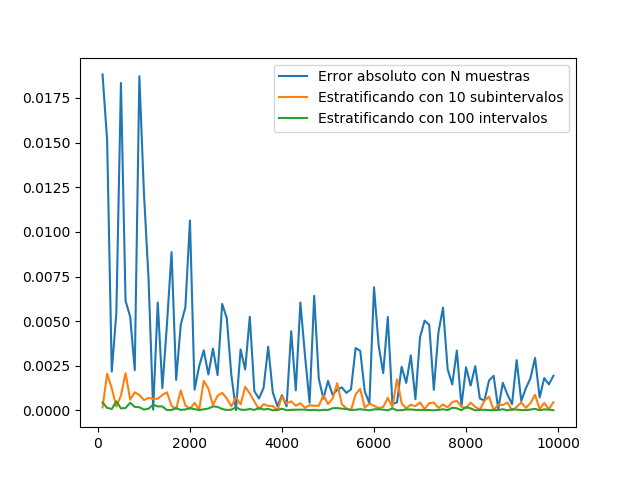
\includegraphics[width=0.6\textwidth]{error_estratificando}
	\caption{Valores de los errores absolutos originales, estratificando con $10$ subintervalos y estratificando con $100$.}
	\label{fig:strat}
\end{figure}

Como mencionábamos, la diferencia es notable. En concreto, el error final estratificando con $100$ intervalos es $0.000014$, dos órdenes de magnitud por debajo del error original. Recordemos que el número de muestras es exactamente el mismo, solo las hemos generado con otra distribución.

La importancia de los errores trasladada a nuestro problema original de renderización de imágenes se traduce en ruido en la imagen. Este ruido impide crear un producto de calidad, por lo que es necesario reducirlo al mínimo. Para cualquier tipo de uso, el caso óptimo serías conseguir mejores resultados sin tener que aumentar el tiempo de cálculo (que en este caso depende directamente del número de muestras usadas).

%Concepto importante pero que no se implementa
\section{Muestreo por importancia (Importance Sampling)}
De la misma forma que en la sección anterior veíamos estratificación como un método de mejora de la integración por Monte-Carlo, en esta sección veremos el muestreo por importancia o \textit{importance sampling}. El objetivo es, de nuevo, reducir la varianza del muestreo. En este caso nos aprovecharemos de que hay variables que tienen más impacto en el valor final de la función que queremos aproximar que otras, por lo que si conseguimos poner énfasis en ellas y muestrearlas con más frecuencia, conseguiremos reducir la varianza. Partimos por lo tanto de una distribución sesgada hacia valores con más impacto, o más importantes, a los que daremos preferencia, de ahí el nombre del método.

El origen del método proviene de problemas con integrales de funciones que son constantes salvo en una pequeña porción del dominio en el que están siendo integradas, por lo que muestrear de forma uniforme no tiene sentido, las muestras deberían concentrarse donde $f$ varía más. Aunque no vamos a tratar detalles específicos del método, tanto en \cite{RestOfYourLife} como en \cite{owen} se pueden ver los desarrollos teóricos detrás del procedimiento. Un dato en concreto que puede ser de ayuda es que cuanto más se parezca la función de densidad de probabilidad de las muestras a la función $f$, menor varianza obtenemos. Para generar puntos aleatorios sobre una función de densidad, aplicamos el método del muestreo con la transformada inversa, tal y como se explica en \cite{RestOfYourLife}, que consiste en generar puntos con $P^{-1}(u)$, donde $u$ es una uniforme en $[0,1]$ y $P$ es la función de distribución de la función de densidad de la que partíamos. 

Es cierto que en el problema general no es posible conseguir una función de densidad de probabilidad exactamente igual a $f$, ya que en las aplicaciones reales no solemos tenerla de forma explícita y suele ser complicada de calcular, por lo que nos contentamos con aproximaciones. Sin embargo, en nuestro caso de ejemplo, para ver cómo afecta este método con varias funciones a nuestro error, sí que sabemos $f$. En la figura \ref{fig:importance} podemos ver los errores absolutos con diferentes funciones de densidad. Aparte de la función constantemente $1$, equivalente a aplicar Monte-Carlo directamente y creada para poder comparar, el resto de funciones de densidad han sido escogidas por ser monótonas decrecientes desde $1$ hasta $0$, al igual que $f$. Notamos que ni la recta ni la función coseno nos proporcionan resultados mejores que un Monte-Carlo directo, al menos no de forma notable. Por otro lado, coger la función $f$ nos deja el error a $0$ desde las primeras muestras. Si conseguimos aproximar $f$, podremos conseguir esta reducción del error.

\begin{figure}[ht]
	\centering
	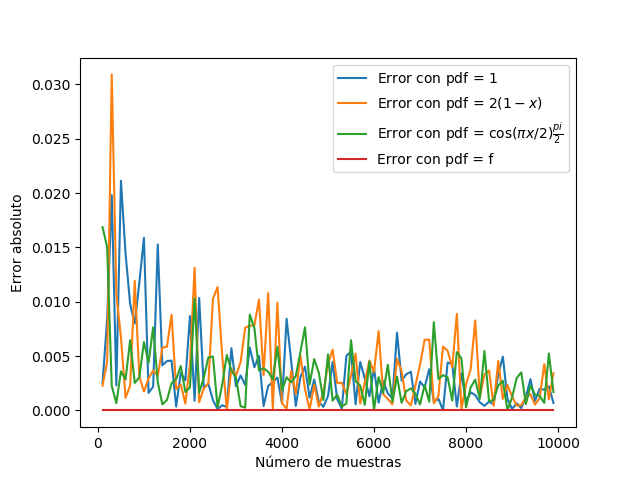
\includegraphics[width=0.6\textwidth]{importancesampling}
	\caption{Errores absolutos con diferentes funciones de densidad a la hora de aplicar \textit{importance sampling}. La función $f$ es la que queremos integrar. }
	\label{fig:importance}
\end{figure}

Es importante notar que, debido a cómo funciona el método del muestreo de la transformada inversa, es necesario calcular una aproximación de la inversa de una función arbitraria en tiempo de ejecución. Esto requiere muchos cálculos, así que es necesario estimar cuánto nos ayuda este \textit{importance sampling} frente a lo que gastamos. En la implementación del ejemplo se ha realizado mediante la librería \textit{pynverse} de Python, que requiere numerosas evaluaciones de la función de distribución antes de devolvernos una buena aproximación de su inversa en un punto dado.

\section{Rechazo de muestras}
\label{rechazo}
El concepto del rechazo de muestras es lo suficientemente común en este tipo de trabajos como para que se vea importante explicarlo a continuación. Es, sin embargo, algo a evitar siempre que sea posible. El algoritmo consiste en muestrear $B \subset A$ mediante una distribución creada sobre $A$, el conjunto que contiene a nuestro objetivo. Todas las muestras contenidas en $A-B$ se ignoran, y solo hacemos los cálculos con aquellas que estén contenidas en $B$.

Puede haber muchas razones para realizar este proceso, pero principalmente suele ser que: la distribución en $A$ es fácil de calcular pero en $B$ no, pero sí que tenemos una función de pertenencia en $B$. Un ejemplo sencillo de esto puede ser obtener una distribución uniforme en un disco a partir de la uniforme en el cuadrado que lo contiene. En ese caso, $A=[-1,1]^2$ y $B$ sería la bola de centro $0$ y radio $1$. La restricción de una distribución uniforme continúa siendo uniforme, por lo que no hay problema en ignorar aquellas muestras tales que $x^2+y^2 > 1$. Sin embargo, es fácil notar que estaríamos usando solo un porcentaje de $\frac{|B|}{|A|}$ muestras, mientras que el resto de $1-\frac{|B|}{|A|}$ serían cálculos malgastados. En nuestro ejemplo, la eficacia del algoritmo sería $\pi/4$. Obteniendo la uniforme en el disco de forma directa (usando por ejemplo coordenadas polares y modificando la longitud de los puntos con la raíz cuadrada, como se verá en la sección \ref{discos}), podemos conseguir el cien por cien de eficacia, sin tener que ignorar ninguna muestra. Es por esto que decíamos anteriormente que este proceso es mejor evitarlo, siempre que sea posible.

Por otro lado, es cierto que a veces no compensa. A lo largo del trabajo veremos ejemplos de rechazo de muestras. En concreto, cuando muestreamos de forma directa una luz, para intentar aplicar \textit{importance sampling}, debido a que las luces son las que más afectan al color de un punto de la escena, nos dedicaremos a generar un punto aleatorio de la luz y compensar el valor que aporta con respecto a la función de densidad en la semiesfera de direcciones. En este proceso se aplica rechazo de muestras en dos ocasiones: la primera es si el punto generado no cae en la semiesfera superior de direcciones del punto, en cuyo caso el rayo no puede llegar de forma directa; la segunda es cuando hay un objeto entre el punto generado en la luz y donde se originó el rayo, en cuyo caso el objeto causaría una sombra y, exceptuando objetos translúcidos, la muestra se ignoraría ya que no aportaría radiancia alguna. La razón de que no usemos distribuciones que contengan estos cálculos ya hechos es que sería demasiado costoso comprobar ambas. En el primer caso, si restringimos la luz solo a la semiesfera superior de direcciones, nos queda un objeto completamente distinto. Uno puede pensar en el caso más simple de luces rectangulares. Restringir a una semiesfera de direcciones es equivalente a cortar con un plano el espacio, y si cortamos con un plano un rectángulo podemos llegar a tener un cuadrilátero genérico o un triángulo. Todos los cálculos que hubiésemos realizado para obtener la función de densidad correspondiente al rectángulo habría que actualizarlos. En el caso del muestreo por área, que veremos en posteriores secciones, quizá no hubiera mucho problema, pero en el muestreo por ángulo sólido se complica considerablemente, todo teniendo en cuenta que tampoco se espera ganar mucho en eficacia debido a que estos casos de rechazo no deberían ser muy habituales en general. En el segundo caso, la sombra que proyectan los objetos de la escena con las luces varía entre cada luz, cada punto en el que se originen los rayos y cada material de los objetos, por lo que los cálculos habría que actualizarlos en cada uno de los rayos. La generación de sombras es un problema complejo por sí solo (de hecho, aplicando algoritmos basados en path-tracing conseguimos resolver este problema de una forma más simple), por lo que no merece la pena gastar tiempo en cálculos.

Con todo ello, este proceso de ignorar parte de las muestras es cómodo pero peligroso en ciertas situaciones. Cuando pensemos que hay alguna forma de sustituirlo por un muestreo directo sin gastar mucho tiempo de cálculo, deberíamos sustituirlo. 

\section{Implementación base}
\label{Implementacion}
La implementación base que se ha usado en este trabajo es la que se construye en \cite{Weekend} y \cite{NextWeek}. Todo lo que tiene relación con ray-tracing (la cámara, los rayos, la intersección con los objetos, objetos básicos como la esfera o planos rectangulares) ya venían creados en este código, que se encuentra abierto. Todo lo que se añade nuevo para los experimentos se detalla en el capítulo \ref{Experimentos}.

Algunos detalles que se han visto en este capítulo que no se encuentran en la implementación son los medios participativos, propagación de rayos y la estratificación a la hora de muestrear. Sí que hay una versión de muestreo por importancia a la hora de muestrear las luces de forma directa, de esto se hablará con más detalle en el capítulo \ref{lucesdir}. También hay materiales de los tipos más básicos, desde superficies lambertianas, que reflejan la energía de forma uniforme en todas las direcciones, superficies de metal con reflejos, y superficies dieléctricas con rayos refractados y reflejados. En general, lo suficiente como para poder crear los experimentos de la forma más simple posible. Si el lector quisiera entrar en contacto con un raytracer más complejo que el que aquí se crea (con mayor separación en clases, mayor potencia y flexibilidad), puede encontrarlo en el código abierto de \cite{pbrt}.


\begin{figure}[ht]
	\centering
	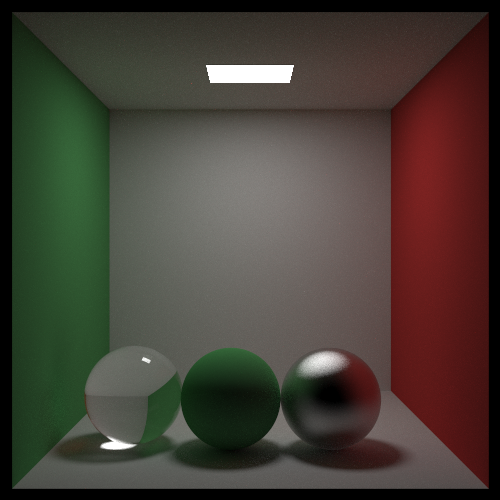
\includegraphics[width=0.6\textwidth]{material_ex}
	\caption{Imagen con un objeto de cada tipo de material, se ha cogido la caja de Cornell y se han insertado esferas con distintos materiales. De izquierda a derecha: dieléctrico, lambertiano y metal. También se puede ver una luz rectangular con material de emisión difusa.}
	\label{fig:mat}
\end{figure}

Hacemos una breve recopilación de las características del programa:
\begin{enumerate}
	\item La imagen final se crea como archivo ppm, uno de los formatos más simples a la hora de escribir imágenes ya que solo necesita los valores finales en los píxeles. No es recomendable en general, debido a que ocupa más de lo que debería.
	\item Vectores de $\mathds{R}^3$ modelados como tres float, hay que notar que double no incrementa la precisión de forma notable en informática gráfica y aumenta los tiempos de cálculo.
	\item Modelo básico de cámara en \textit{camera.h}. Se definen con su objetivo, posición, vertical (que indica el inclinamiento de la cámara), campo de visión, relación de aspecto de la imagen final y distancia al foco.
	\item Modelo de rayos en \textit{ray.h}, se definen con un punto origen y su vector dirección.
	\item Los objetos, definidos en el archivo \textit{hittable.h} se caracterizan por tener cuatro funciones, dos de ellas, \textit{random} y \textit{pdf\_value}  relacionadas con muestrear luces de área, que veremos en la sección \ref{lucesdir}. Las otras dos referentes a la intersección con rayos: \textit{hit} que comprueba si un rayo interseca el objeto, guardando información de la intersección como la distancia, punto de corte, normal de la superficie en el punto (para calcular la iluminación en el punto), y el material de la superficie en caso de que lo tuviera; y \textit{bounding\_box}, que se utiliza para agrupar objetos en ortoedros jerárquicos, que son más simples de manejar, con el simple objetivo de filtrar aquellos rayos que ni siquiera intersecan el ortoedro, ya que entonces es imposible que intersequen al objeto en sí. Estos ortoedros jerárquicos vienen definidos en \textit{box.h} y \textit{bvh.h}.
	\item Se pueden tener listas de objetos agrupados, definidas en \textit{hittable\_list.h}.
	\item Hay dos objetos creados, las esferas en \textit{sphere.h} y los rectángulos perpendiculares a algún vector de la base usual, en \textit{aarect.h}. En el trabajo hemos visto necesario añadir las elipses con cualesquiera dos semiejes, incluidas en \textit{elipses.h}. 
	\item Los materiales básicos, definidos en \textit{material.h}, son:
	\begin{itemize}
		\item Lambertiano, que refleja de forma uniforme en todas las direcciones. 
		\item Metal, que refleja con parte de aleatoriedad. Esta aleatoriedad depende de un parámetro del material denominado \textit{fuzz}, que con valor bajo da lugar a rayos especulares, con ángulo igual al de incidencia, como un espejo, y con valor alto causa reflexión difusa.
		\item Dieléctrico, utilizado principalmente para simular cristal. Es un material con parte de rayos reflejados y parte refractados.
		\item Emisión difusa, utilizado para simular luces de área.
	\end{itemize}
	
	En la figura \ref{fig:mat} se ha incluido una imagen con una esfera por cada tipo de material junto a una luz de área rectangular en el techo, para poder ver cada tipo de material. También soporta texturas, definidas en \textit{texture.h}, pero no las usaremos en los experimentos.
	\item Por otro lado, en la figura \ref{fig:estructura} se ha añadido un esquema del funcionamiento general del \textit{main}, de la forma más simplificada posible. Nótese que solo tiene una función vital, que es la función \textit{color}. Todos los ficheros y las clases solo son soporte de la generación de los rayos iniciales y de esta función. 
\end{enumerate}

\begin{figure}[ht]
	\centering
	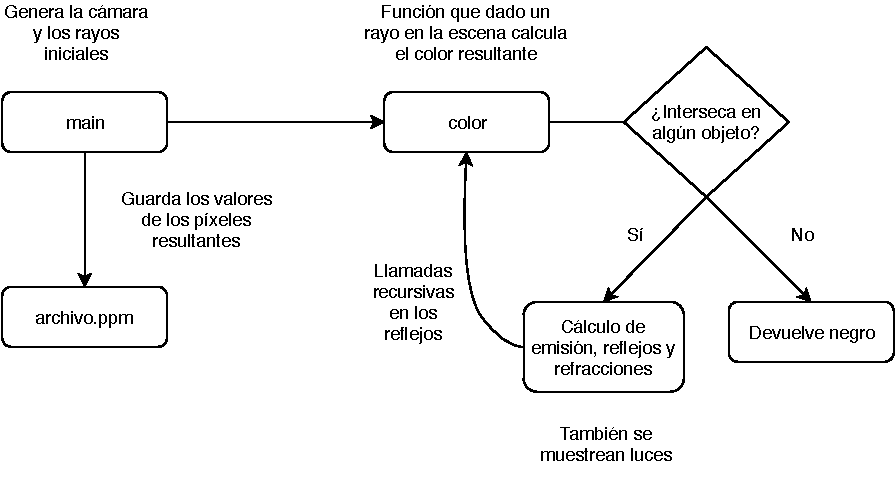
\includegraphics[width=0.6\textwidth]{estructurageneral}
	\caption{Estructura general del main del programa. Nótese la importancia de la función \textit{color}, que prácticamente hace todo el trabajo. Los detalles de cálculo de emisión y reflexión se hacen en base a lo explicado en las anteriores secciones.}
	\label{fig:estructura}
\end{figure}

Si bien esto es referente al código base, en el anexo \ref{anexo} se puede consultar el código original creado para este trabajo, en el que se ha intentado comentar las partes importantes del mismo.

\chapter{Luces de área y tipos de muestreo}

\label{lucesdir}
En el apartado anterior hemos descrito cómo funciona la renderización realista con métodos basados en path-tracing, cómo resolver una ecuación integral está íntimamente conectado a conseguir buenos resultados y los métodos principales usados para aproximar la solución. En este apartado vamos a tratar de entrar más a fondo en el muestreo de luces de forma directa y las diferentes formas a la hora de hacerlo. Si el capítulo anterior eran las bases para entender el problema, este capítulo expone la esencia del muestreo de luces y sirve de introducción necesaria a los experimentos y resultados que veremos en el capítulo \ref{Experimentos}.

Si recordamos en la sección \ref{rendering} introducimos la ecuación de renderización que usamos para hallar cuánta radiancia obtiene un punto del mundo, y dependía de una integral sobre una semiesfera de direcciones y que sumaba la radiancia obtenida de cada una de las direcciones. De forma natural, las luces de la escena generan más radiancia que el resto de puntos. Aplicando muestreo por importancia, podemos pensar que nos conviene encontrar una función de densidad de la semiesfera que tenga más valor en los rayos hacia las luces. Este método viene explicado con detalle en \cite[Secciones~6-9]{RestOfYourLife}. 

La idea principal es que la combinación convexa de funciones de densidad seguirá siendo una función de densidad, por lo que podemos usar dos: una que muestree de forma directa las luces, y otra que se encargue del resto de direcciones. Es importante que la función de densidad final no sea cero en ninguna región de la semiesfera, para mantener la convergencia de la imagen final. Por lo que mezclando una función de densidad no negativa solo en la luz junto a una uniforme en todas las direcciones, conseguimos aplicar muestreo por importancia. La diferencia entre los posibles métodos radica en qué función de densidad escogemos para cada luz.

En la siguiente sección veremos las dos posibilidades principales que luego utilizaremos en el capítulo \ref{Experimentos}, muestreo en función del ángulo sólido frente al del área.



\section{Muestreo por ángulo sólido y muestreo por área}
\label{areaangulo}
La forma más simple de muestrear de una luz es una distribución uniforme en su superficie. La función de densidad en la propia superficie será $\frac{1}{A}$ donde $A$ es el área. Es necesario entender que esta no es la función de densidad que necesitamos para aplicar Monte-Carlo, ya que la integral de la ecuación de renderización es sobre la semiesfera de direcciones. Es decir, necesitamos saber la función de densidad de esa superficie en la proyección en la semiesfera. En el caso de una luz plana rectangular, por ejemplo, se nota en  \cite[Sección~9]{RestOfYourLife} que la función de densidad en la semiesfera es:
\begin{equation}\label{eq:area}
p(\text{direccion(p,q)}) = \frac{d(p,q)^2}{\cos(\alpha)A},
\end{equation}
donde $p$ es el centro de la semiesfera, $q$ el punto que hemos muestreado de la luz, $d$ es la función distancia en $\mathds{R}^3$ y $\alpha$ es el ángulo entre $q-p$ y el normal del rectángulo. Debido a que muestreamos de forma uniforme en el propio rectángulo, esto es lo que denominamos muestreo por área, ya que la probabilidad de que se obtenga una región depende directamente de su área.

El método entonces consiste en muestrear un punto de forma uniforme en la luz, ver si hay objetos en el rayo con origen el punto al que calculamos la radiancia y destino el punto muestreado, y en cuyo caso ignorar el rayo por completo, y dividir el resultado obtenido por la probabilidad de muestrear este rayo, que nos lo da la función de densidad sobre la semiesfera de direcciones. Esta forma simple de conseguir muestrear una luz de forma directa tiene algunos fallos. En particular, en la figura \ref{fig:areasolid} se puede observar en la parte izquierda del diagrama un ejemplo de este tipo de muestreo. Cuando las luces que muestreamos son grandes, empezamos a ver ciertos conjuntos de rayos muestreados muy cerca entre sí. Esto significa que se generarán más rayos en estas regiones que otras. Si bien la distribución era uniforme en la luz, dejó de serlo cuando proyectamos sobre la esfera. Como también viene en el diagrama en la parte de la derecha, una forma de resolver esto es muestrear en función del ángulo sólido. Es decir, que la distribución sea uniforme en la proyección de la semiesfera.

\begin{figure}[ht]
	\centering
	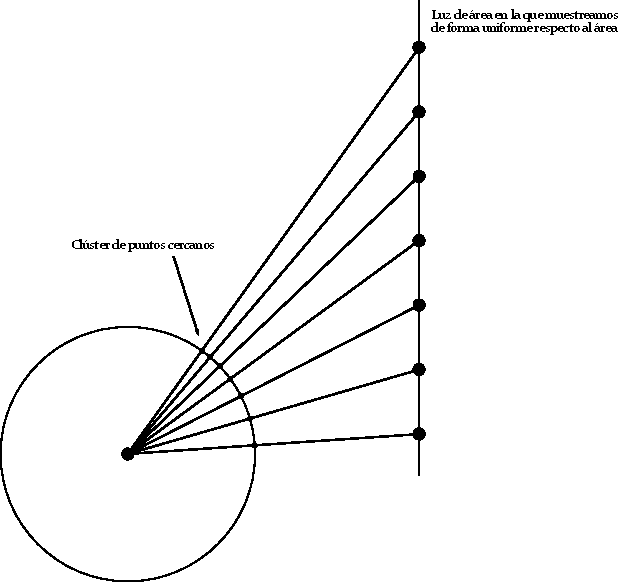
\includegraphics[width=0.45\textwidth]{area}
	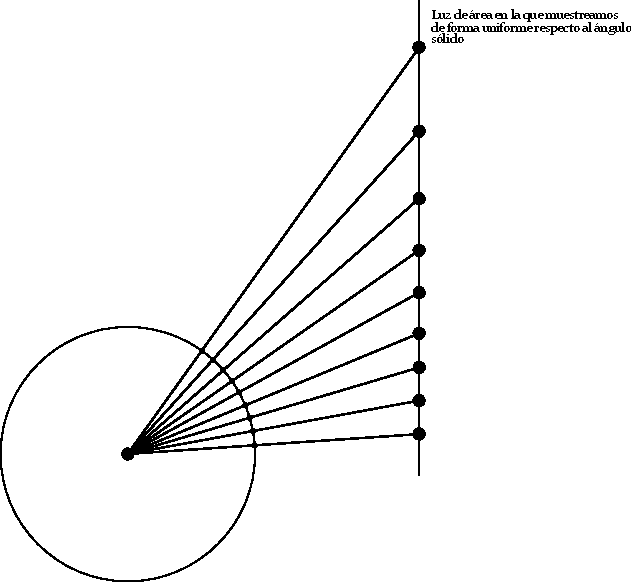
\includegraphics[width=0.45\textwidth]{solid_angle}
	\caption{Muestreo de una luz de área simplificado. A la izquierda cada punto se muestrea en función del área, y a la derecha en función del ángulo sólido. Cuando los puntos de muestra son uniformes en la luz, se crean conjuntos unidos o clústers de puntos en la esfera de direcciones del punto de vista de partida, lo que significa que creamos varios rayos más juntos de lo normal. Esto desaparece si muestreamos uniformemente bajo el ángulo sólido, que implica que puntos más lejanos estarán más repartidos en la luz, debido a que afectan menos en nuestro punto. }
	\label{fig:areasolid}
\end{figure}

El problema es que muestrear en función del ángulo sólido no es para nada sencillo. En el capítulo \ref{Experimentos} implementamos varios algoritmos de la última década para conseguir muestrear en función del ángulo sólido luces rectangulares y discos. Nótese que es necesario un algoritmo específico para cada tipo de luz, por lo que es fácil de imaginar la complejidad de este método. Sin embargo, la capacidad de reducir la varianza de la muestra, y por tanto disminuir el error hace que merezca la pena investigarlo.

\chapter{Experimentos y resultados}
\label{Experimentos}

Para intentar estudiar la diferencia entre el muestreo por ángulo sólido y por área, se han implementado tres algoritmos de muestreo en luces particulares: luces rectangulares y discos. Estos algoritmos están basados en \cite{ur2013}, \cite{ur2017} y \cite{ur2018} respectivamente. Es importante notar que las parametrizaciones que se crean en estos tres artículos no solo sirven para muestrear en función del ángulo sólido, si no que son útiles para otras aplicaciones. Aquí, sin embargo, solo vamos a tratar este uso.
%Mis graficasssssss, la más importante es la que habla del aumento de eficacia a la hora de tener luces más grandes
\section{Luces rectangulares}
\label{lucesrectangulares}
A continuación veremos los resultados de aplicar los dos tipos de muestreo, por área y por ángulo sólido, a luces rectangulares. El muestreo por área se consigue generando un punto $X = p_0 + u_1(p_1-p_0)+u_2(p_3-p_0)$ suponiendo que el rectángulo está formado por los puntos $p_i, i=0,\hdots,3$ y con $u_i, i =1,2$ siendo dos puntos generados por una distribución uniforme en $[0,1]$. Usando la función de densidad que produce esta generación uniforme de la luz proyectada en la semiesfera que mencionábamos en \ref{eq:area}, conseguimos muestrear correctamente por área.

Por otro lado, la generación uniforme en función del ángulo sólido se ha implementado siguiendo los pasos descritos en \cite{ur2013}. En la implementación se ha utilizado como base las clases \textit{aarect} de \cite{RestOfYourLife}. Estos objetos describen el comportamiento de rectángulos que son perpendiculares a algún vector de la base usual, que son más simples de describir que en general. En ellos ya estaban definidas las funciones de generación de un punto aleatorio y su respectiva función de densidad, por lo que lo único que se ha hecho para implementar luces rectangulares con generación de rayos directos uniformes en función del ángulo sólido ha sido cambiar estas dos funciones. La función de densidad pasa a ser la constante $\frac{1}{S}$, donde $S$ es el área del rectángulo proyectado en la esfera, justo por ser uniforme respecto al ángulo sólido. Por otro lado, la generación del punto aleatorio es en la que se han seguido los pasos descritos en \cite{ur2013}, creando la función $M:[0,1]^2 \rightarrow Q$, donde $Q$ es la proyección del rectángulo en la esfera de direcciones. Esta función cumple que regiones del mismo área tienen imágenes con mismo ángulo sólido, por lo que una distribución uniforme en $[0,1]^2$ se transforma en una distribución uniforme bajo el ángulo sólido en $Q$. Esta es la propiedad que nos permite realizar este muestreo. Un hecho interesante, que se cumple para los dos algoritmos de muestreo por ángulo sólido que implementamos en esta sección, que se pueden consultar en \cite{ur2013} y \cite{ur2017}, es que la reducción de varianza que otorgan al cálculo de la imagen es mayor en medios participativos que en dispersión de luz. Nosotros solo trataremos este segundo caso, pero cabe mencionar que los errores serían aún menores con escenas conteniendo medios participativos, como por ejemplo aquellas que contengan simulaciones de niebla.

A la hora de ver la eficacia de cada método, se ha creado una imagen original con las mismas dimensiones, pero generando muchas más muestras (un total de 4000). Un ejemplo de la imagen original junto a una de cada uno de los otros métodos se puede ver en la figura \ref{fig:cornell}, donde se ha utilizado la caja de Cornell que venía ya diseñada en \cite{RestOfYourLife}. A simple vista no hay mucha diferencia entre ambos métodos en este escenario, no es de extrañar debido a que la mejora que estamos aplicando reduce solo un poco el error, y que la luz, en este caso, no es especialmente grande, ya vimos en la sección \ref{areaangulo} que la diferencia entre ambos muestreos se nota más cuando más amplia es la luz. Esta hipótesis teórica también la comprobaremos en los experimentos. 

\begin{figure}[ht]
	\centering
	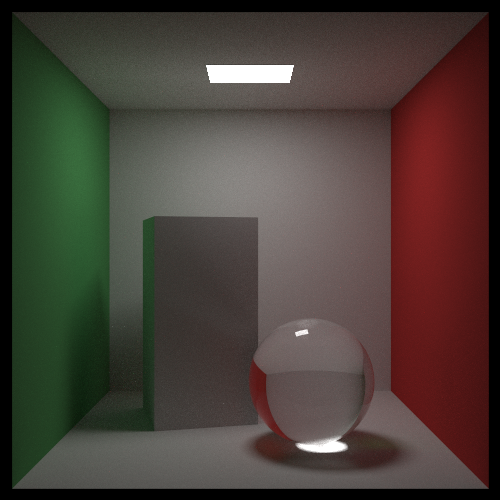
\includegraphics[width=0.3\textwidth]{original}
	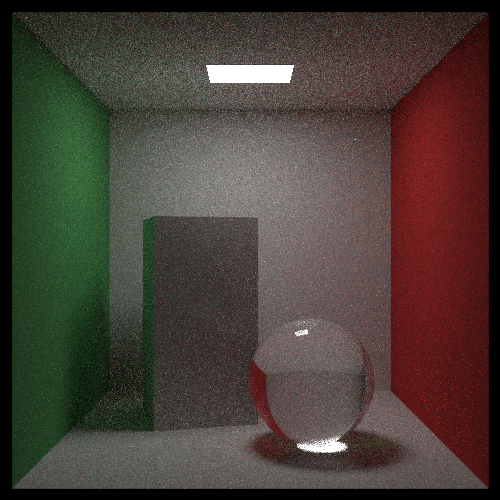
\includegraphics[width=0.3\textwidth]{area_20}
	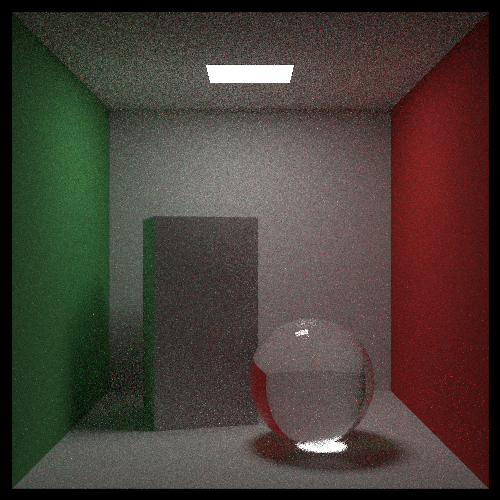
\includegraphics[width=0.3\textwidth]{solidangle2_20}
	
	\caption{De izquierda a derecha: imagen original utilizada como modelo para comparar creada con 4000 muestras por píxel; imagen generada con muestreo uniforme en función del área, creada con 100 muestras por píxel; imagen generada con muestreo uniforme en función del ángulo sólido,  creada con 100 muestras por píxel.}
	\label{fig:cornell}
\end{figure}

Se han creado unas veinte imágenes con cada modelo, variando el número de muestras por píxeles, para ver cómo evoluciona cada uno frente a más muestras y la diferencia entre ambos, variando linealmente desde cinco hasta cien muestras por píxel. A cada una de las imágenes se le ha aplicado la raíz del error cuadrático medio con los valores de la imagen original. Las gráficas de estos errores se pueden ver en la figura \ref{fig:graficasbasic}. Notamos que el método de muestreo uniforme en función del área es más rápido pero tiene un ligero incremento de error. Esto es esperable debido a que los cálculos para muestrear por área son más simples y rápidos.

\begin{figure}[ht]
	\centering
	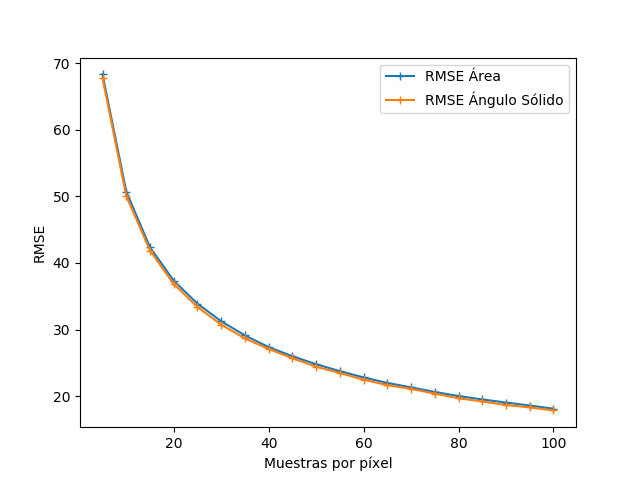
\includegraphics[width=0.45\textwidth]{rmse_basicv2}
	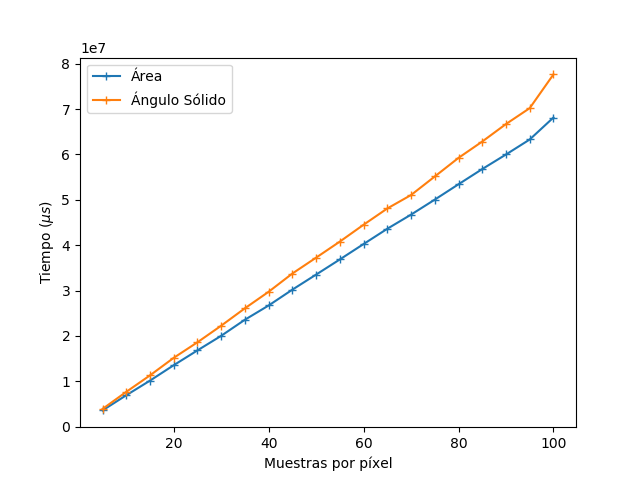
\includegraphics[width=0.45\textwidth]{tiempo_basicv2}
	
	\caption{A la izquierda podemos ver la gráfica con la raíz del error cuadrático medio de las veinte imágenes experimento con cada método, tomada en función de la imagen original de 4000 muestras. A la derecha está el tiempo en micro segundos de cada ejecución.}
	\label{fig:graficasbasic}
\end{figure}

Por otro lado, como también nos interesa comprobar que este efecto es mayor conforme más grande es la luz (debido a que los rayos tienden más al borde cuando se muestrea de forma uniforme con el área, como ya vimos anteriormente), se ha comprobado con el mismo escenario, solo que aumentando el tamaño de la luz rectangular. En la figura \ref{fig:graficasgrande} se puede comprobar tanto la imagen nueva, para ver el cambio, como los valores de los resultados con este nuevo escenario, tanto de error como en tiempo. También se puede ver la diferencia de los errores entre los métodos en ambos experimentos (nótese que los valores positivos significan que el error con ángulo sólido es menor). Esta última gráfica es la que nos indica que, en efecto, cuando hemos ampliado la luz los errores del método de área son mucho mayores. Esta diferencia disminuye cuantas más muestras por píxel hagamos debido a que ambos métodos acaban convergiendo a la imagen final, por lo que la diferencia entre los errores debería converger a cero. Pero es interesante ver que lo que ganamos con el nuevo método es el doble aún con cien muestras por píxel en el nuevo escenario. Esto sugiere que, de cara a un problema práctico, sería posible cambiar entre métodos dependiendo de el tamaño relativo de las luces frente a los objetos. Por otro lado, en ambos experimentos hemos visto que muestrear por el ángulo sólido conlleva entre un 10\% y un 15\% más de tiempo en cálculos, dependiendo de la situación puede ser crítico, si los tiempos de cálculo duran semanas, o no importar.



\begin{figure}[ht]
	\centering
	\begin{align}
	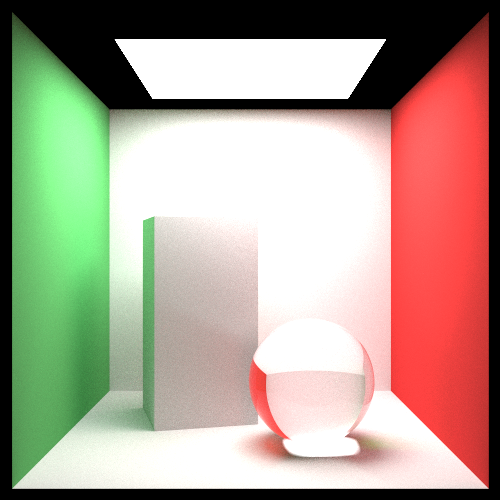
\includegraphics[width=0.3\textwidth]{original_grande}
	\hspace{1cm}&
	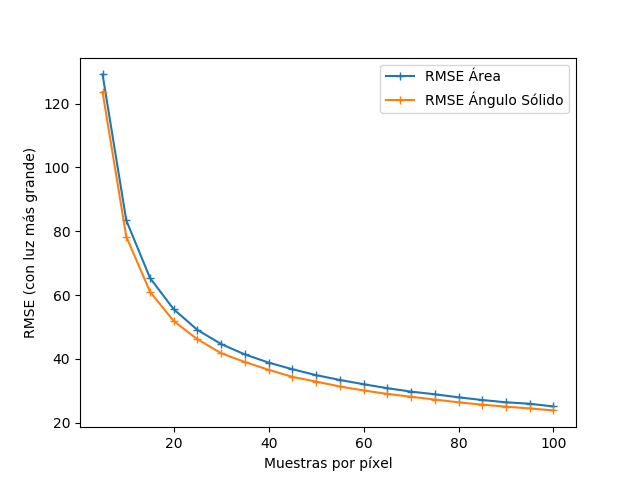
\includegraphics[width=0.45\textwidth]{rmse_luz_grande}\\
	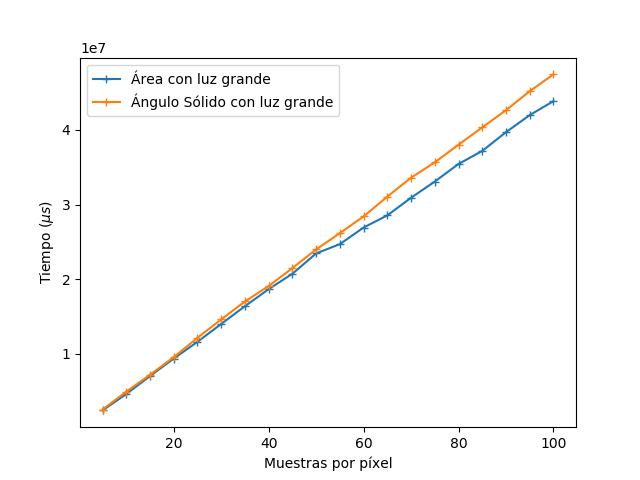
\includegraphics[width=0.45\textwidth]{tiempo_grandev2}&
	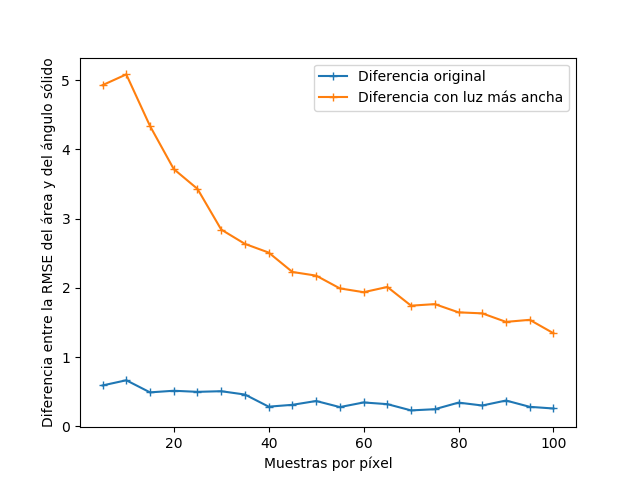
\includegraphics[width=0.45\textwidth]{diferencia_luz_grandev2}\\
	\end{align}
	
	\caption{Arriba se encuentra la nueva imagen modelo, en la que se ha ampliado la luz rectangular. Arriba a la derecha se encuentra la gráfica de los errores con ambos métodos, abajo a la izquierda los tiempos de las ejecuciones y abajo a la derecha la diferencia entre los errores de los métodos en ambos experimentos.}
	\label{fig:graficasgrande}
\end{figure}

Otro aspecto a notar de las gráficas es que muestrear la imagen con la luz más grande ha resultado en la mitad de tiempo de cómputo, con la misma resolución y muestras por píxel. Esto puede ser consecuencia de que la probabilidad de que un rayo acabe en la luz es más alta, por lo que es más fácil que los rayos generados con la segunda función de densidad, aquella que muestreaba en toda la semiesfera de direcciones, intersequen a la luz y finalicen el cálculo. Cuando no ocurre esto, tienen que hacer múltiples llamadas recursivas a la función \textit{color} que describíamos en \ref{Implementacion} por lo que los tiempos aumentan. 

Es importante notar que en escenas complejas, se tardan varios órdenes de magnitud más de tiempo en calcular sombras en cada rayo que en generarlos. Esto implica que, si podemos reducir la varianza de cada rayo con este tipo de métodos, nos va a merecer la pena aunque perdamos algo más de tiempo en la generación de rayos. Esto no ocurre en nuestra escena porque es demasiado simple.

\section{Discos}
\label{discos}
En esta sección veremos cómo afecta cada tipo de muestreo cuando tratamos luces en forma de disco. Debido a que no se encontraban implementados en \cite{RestOfYourLife} como objeto, se han implementado y se adjuntan en el archivo \textit{ellipses.h}, donde se han implementado elipses en general con cualesquierda dos semiejes. En particular, cuando queremos discos solo tenemos que usar semiejes de la misma longitud. Esta implementación base utiliza la generación de puntos en función del área. En este caso la generación de puntos aleatoria se ha conseguido con $X = c + \sqrt{\rho}\cos(\phi)a_1 + \sqrt{\rho}\sin(\phi)a_2$, donde $\rho$ es un punto aleatorio obtenido de una distribución uniforme en $[0,1]$, $\phi$ es un punto aleatorio obtenido de una distribución uniforme en $[0, 2\pi]$ y $a_1, a_2$ son los semiejes del disco. Lo único que hemos hecho ha sido tratar el disco como $[0,1]\times[0,2\pi]$ y trabajar en coordenadas polares. Es importante notar que la raíz cuadrada es necesaria para que los puntos sean en efecto uniformes en el disco, lo cual se puede comprobar realizando el determinante del jacobiano de la transformación:
$$\begin{vmatrix}
\frac{\cos(\phi)}{\sqrt{\rho}} \frac{1}{2} & \frac{\sin(\phi)}{ \sqrt{\rho}}\frac{1}{2} \\
-\sqrt{\rho}\sin(\phi) & \sqrt{\rho}\cos(\phi)
\end{vmatrix} = \frac{1}{2},$$
que es constante. Si no hubiésemos usado la raíz cuadrada, saldría en función de $\rho$ por lo que la aplicación cambiaría la función de densidad.

Como nota adicional, cuando hablamos de elipses esféricas nos referimos a la proyección del disco sobre la esfera, no al disco en sí. Como cada disco tiene asociada una elipse, es posible que a lo largo del trabajo utilicemos ambos términos para referirnos a una proyección concreta.

Por otro lado, la generación de puntos en el disco uniformes respecto al ángulo sólido se ha hecho en el archivo \textit{ellipsessa.h}. Al igual que con las luces rectangulares, la función de densidad es fácil de calcular ya que es solo $\frac{1}{S}$, donde $S$ es el área del disco proyectado en la esfera de direcciones. Como este valor es necesario en el algoritmo de generación de un punto aleatorio, simplemente la guardamos en una variable para usarla en la función de densidad. Para la generación del punto en sí, se ha implementado el algoritmo descrito en \cite{ur2017}, en concreto el denominado \textit{parallel mapping}. Al contrario que en la sección anterior, hay que remarcar ciertas diferencias en la implementación usada aquí respecto a la descrita, que naturalmente afectan a los resultados y a las conclusiones. Primero de todo, el algoritmo depende de una función $\Omega_d$, descrita como una integral. Esta función describe el ángulo sólido de una región del disco proyectado en la esfera, por lo que es vital a la hora de realizar los cálculos posteriores. Sin embargo, la integral no tiene forma cerrada, por lo que depende de cálculos numéricos varios. En nuestra implementación en lugar de realizar los cálculos propuestos sobre la integral, se ha optado por calcular la integral original con la regla de Simpson compuesta, de forma que tenemos flexibilidad a la hora de elegir cuánta precisión queremos frente al cálculo utilizado, y creemos que simplifica bastante el procedimiento. En el artículo original se propone una expresión que depende de integrales elípticas incompletas. Por otra parte, es necesario hallar la raíz de una función que depende de $\Omega_d$ también con cálculos numéricos, y aunque se recomienda el método de Newton-Raphson, en este trabajo hemos usado el método de la bisección. De nuevo, simplifica los cálculos, pero es muy posible que cause mayores tiempos de los usuales. Como nos interesaba principalmente la diferencia en los errores y en la varianza, no hemos visto que cambiar estos métodos cambie mucho las conclusiones, pero el lector debería ser consciente de estos detalles.

Al igual que en la sección anterior, se han realizado cuatro conjuntos de ejecuciones: una ejecución con luz de disco con distribución en función del área, otra en función del ángulo sólido y otras dos cambiando el tamaño de la luz. De nuevo, queremos ver la diferencia entre los muestreos respecto al tamaño de la luz. En la figura \ref{fig:cornell_ellipse} se pueden observar tres imágenes: la original, creada con 4000 muestras por píxel y que funciona como modelo de comparación, la creada con la distribución de área y la del ángulo sólido. Al igual que con las luces rectangulares, la diferencia es difícilmente visible, pero luego veremos con más detalle cuánto error tiene cada una. Al igual que antes, se han creado veinte imágenes con cada modelo, variando el número de muestras de píxel desde 5 hasta 100. Se ha conseguido el error cuadrático, en función de la imagen modelo, y el tiempo de ejecución. Es importante notar que estos experimentos se realizan con la función de densidad mixta, juntando la directa con la luz con una uniforme ne la esfera de direcciones. Es decir, que estamos cambiando solo la mitad de esta función al cambiar de modelo. Esto puede explicar parte de la similitud que obtendremos. Se ha realizado de esta manera porque así es como se utilizará luego en renderización, por lo que no tenía sentido experimentar solo con la función de densidad directa a la luz. 

\begin{figure}[ht]
	\centering
	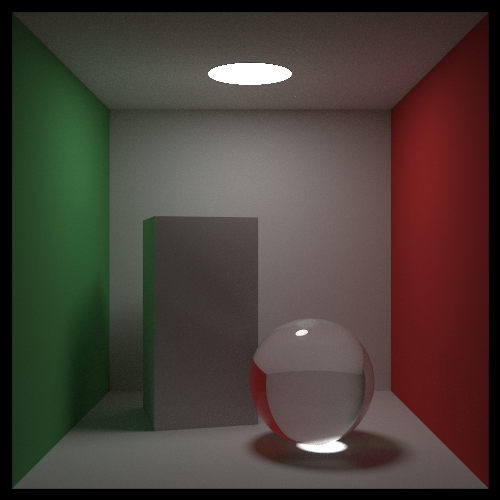
\includegraphics[width=0.3\textwidth]{original_ellipse}
	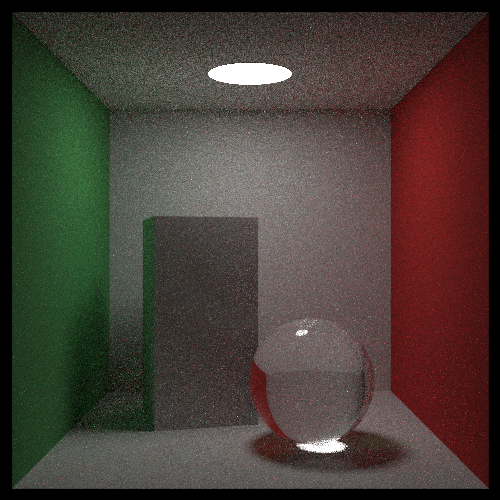
\includegraphics[width=0.3\textwidth]{ellipse_20}
	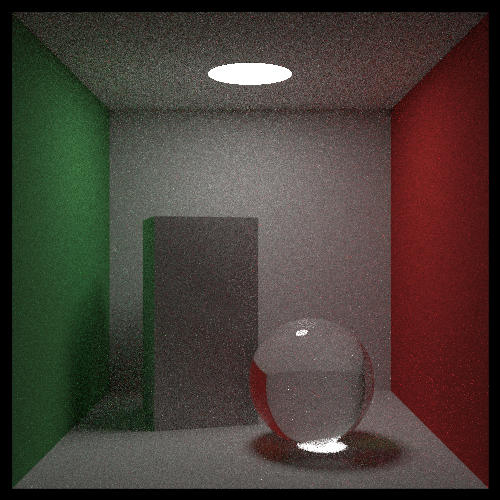
\includegraphics[width=0.3\textwidth]{ellipse_sa_20}
	
	\caption{De izquierda a derecha: imagen original utilizada como modelo para comparar creada con 4000 muestras por píxel; imagen generada con muestreo uniforme en función del área, creada con 100 muestras por píxel; imagen generada con muestreo uniforme en función del ángulo sólido,  creada con 100 muestras por píxel.}
	\label{fig:cornell_ellipse}
\end{figure}

En la figura \ref{fig:elipsesgraficas} podemos observar los errores y los tiempos con el tamaño de luz original. Al igual que con las luces rectangulares, el ángulo sólido funciona con menos error que el área, aunque es difícilmente notable. Por otro lado, la diferencia en el tiempo es más pronunciada con este algoritmo, tardando unas cinco veces más que la generación por área. Esto es debido a lo que hablábamos anteriormente de los cálculos de la integral y la raíz que están incluidos en el algoritmo, que aumentan considerablemente el tiempo de ejecución. De la misma manera, es posible disminuir estos tiempos cambiando los parámetros de los métodos de bisección (cuántas iteraciones se realizan) y de la regla de Simpson (cuántos pasos intermedios se cogen). Esto, naturalmente, aumentaría los errores.

\begin{figure}[ht]
	\centering
	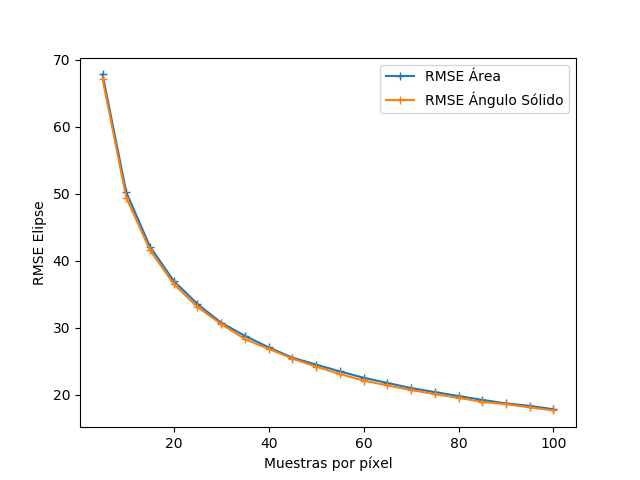
\includegraphics[width=0.45\textwidth]{rmse_elipse}
	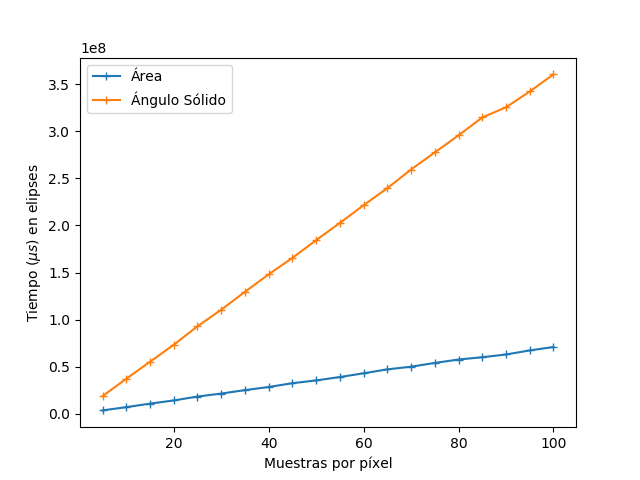
\includegraphics[width=0.45\textwidth]{tiempo_elipse}
	
	\caption{A la izquierda podemos ver la gráfica con la raíz del error cuadrático medio de las veinte imágenes experimento con cada método, tomada en función de la imagen original de 4000 muestras. A la derecha está el tiempo en micro segundos de cada ejecución.}
	\label{fig:elipsesgraficas}
\end{figure}

Por otro lado, en la figura \ref{fig:elipsesgrande} podemos ver el segundo experimento, con una luz el triple de amplia. Los tiempos se mantienen parecidos, con seis veces más de ejecución en el modelo de ángulo sólido que en el de área. El error es más amplio, y se puede ver con más claridad en la última gráfica que denota la diferencia entre ángulo sólido y área. Que los valores sean positivos indican que en efecto disminuimos el error con el nuevo algoritmo, lo que implica menos varianza por cada rayo. Al igual que antes, la diferencia es más amplia en el caso de la luz amplia, lo que implica que si estamos tratando con escenas donde los objetos son pequeños en relación a las luces, nos interesa más el muestreo uniforme respecto al ángulo sólido. 

\begin{figure}[ht]
	\centering
	\begin{align}
	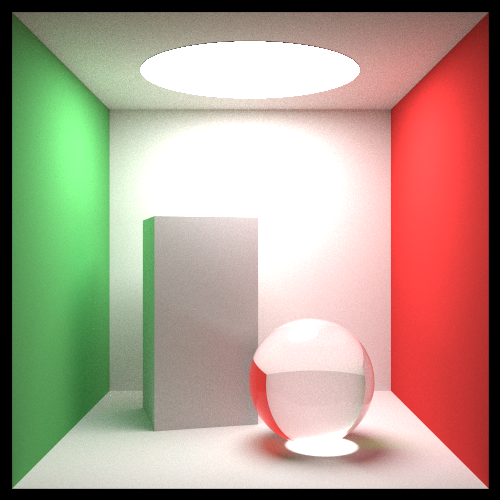
\includegraphics[width=0.3\textwidth]{original_ellipse_grande}
	\hspace{1cm}&
	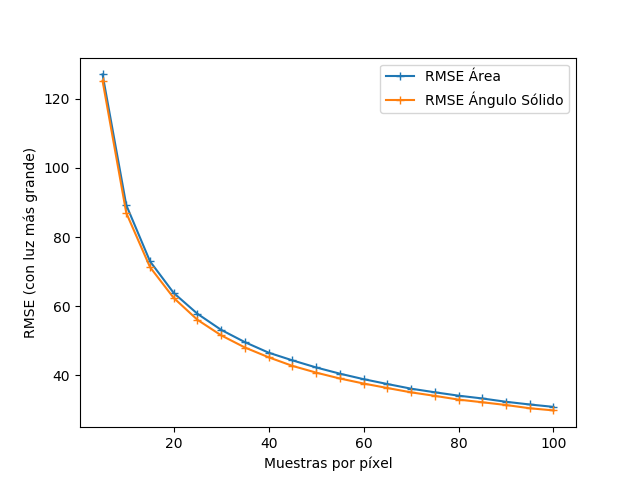
\includegraphics[width=0.45\textwidth]{rmse_elipse_grande}\\
	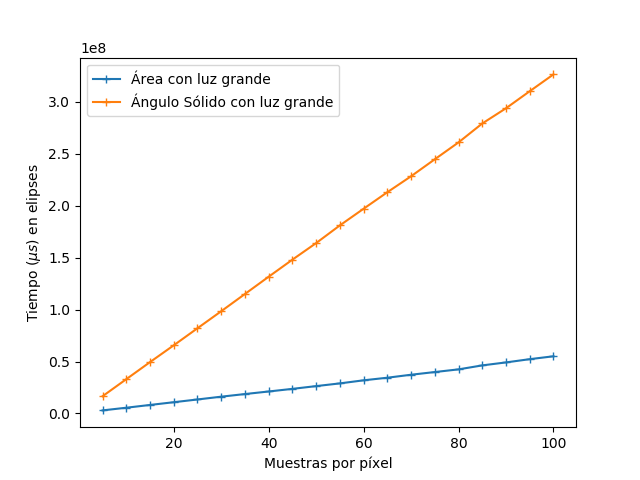
\includegraphics[width=0.45\textwidth]{tiempo_elipse_grande}&
	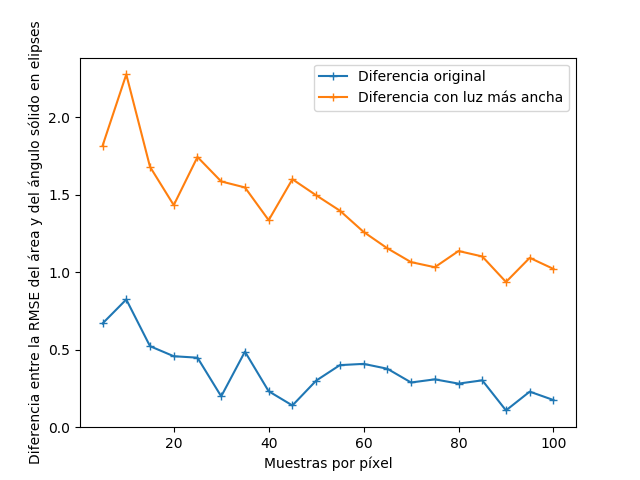
\includegraphics[width=0.45\textwidth]{diferencia_elipse}\\
	\end{align}
	
	\caption{Arriba se encuentra la nueva imagen modelo, en la que se ha ampliado la luz rectangular. Arriba a la derecha se encuentra la gráfica de los errores con ambos métodos, abajo a la izquierda los tiempos de las ejecuciones y abajo a la derecha la diferencia entre los errores de los métodos en ambos experimentos.}
	\label{fig:elipsesgrande}
\end{figure}


%Arv95 con dos triángulos y previous works en general de los papers

\chapter{Conclusiones}
En el trabajo hemos explorado y explicado el uso de muestreo directo en fuentes de luz dentro del algoritmos basados en path-tracing. Tanto la base, su estructura y su implementación concreta, y los detalles que más afectan a la hora del tiempo de ejecución. Usando técnicas descubiertas en la última década, se han expuesto el muestreo de puntos por área y por ángulo sólido en dos de los tipos de luces de área más comunes, rectángulos y discos. Tanto de forma teórica como experimentos prácticos, se ha visto la diferencia entre ambos métodos para cada luz. Hemos tratado de investigar también cómo afecta el tamaño de la luz a los resultados, viendo que tal y como preveíamos, el ángulo sólido es más eficaz cuanto más amplias son las luces de área.

Por último, cabe destacar que en trabajos futuros sería recomendable continuar el estudio con otros tipos de luz. En particular, las proyecciones de casquetes esféricos, cuyo algoritmo de muestreo por ángulo sólido se puede ver en \cite{ur2018}. Otros proyectos podrían tratar también de ver con más detalle cómo afecta en el caso de los discos diferentes algoritmos e implementaciones a la hora de los cálculos numéricos. En nuestro caso hemos usado bisección y la regla de Simpson para resolver los ceros de una función y el valor de una integral sin forma cerrada, respectivamente, pero convendría estudiar si Newton-Raphson mejora los resultados (ya que usamos una evaluación más por iteración con la derivada, pero debería converger antes) o si hay alternativas a la regla de Simpson compuesta usada aquí. También podría estudiarse el resto de algoritmos propuestos en \cite{ur2017} para los discos, ya que solo hemos estudiado el \textit{parallel mapping}, habiendo otras posibilidades.

Otra propuesta, que no hemos visto comentada en las investigaciones pero que quizás podríamos estudiar, es  restringir las direcciones del muestreo de luz directo a la semiesfera superior de direcciones. Como explicábamos en la sección teórica, cada rayo de luz debe originarse en esta semiesfera, que es donde integramos. Sin embargo, a lo largo de los algoritmos de muestreo directo se suele usar la esfera entera por conveniencia de facilidad de cálculos, haciendo rechazo de muestras en aquellas que caen fuera de la semiesfera. Debido a que el rechazo de muestras es malgastar tiempo de ejecución, sería conveniente estudiar si hay alguna forma simple y eficaz de evitar este problema, al menos parcialmente. En luces rectangulares por ejemplo se podría coger el menor rectángulo que contiene toda la región de la semiesfera de direcciones, que seguiría manteniendo rechazo de muestras pero sería menor en otros casos. Esto aumenta el cálculo, por lo que quizá no sea óptimo realizarlo. 




% --------------------------------------------------------------------
% APPENDIX: Opcional
\appendix
\chapter{Código}
\label{anexo}
Como ya se ha mencionado a lo largo del trabajo, la mayoría del código adjunto con este trabajo es obra de Peter Shirley, en particular de su libro \cite{RestOfYourLife}. Sin embargo, ha habido algún par de clases nuevas, necesarias para las elipses o las luces rectangulares con generación de puntos uniforme en función del ángulo sólido, por lo que vemos necesario explicar en este anexo esta implementación. Lo exponemos a continuación según el fichero en el que estén.

Como nota aclaratoria antes del código en sí, para poder ejecutar este código es necesario compilarlo, con una orden usual como 'g++ -o main main.cc', y posteriormente ejecutarlo enviando la salida a un archivo ppm, que es como lo formateó Peter Shirley en su obra original. Por ejemplo, 'main > prueba.ppm'. Un programa con el que abrir este tipo de archivos es GIMP.

\lstset{language=C++}
\definecolor{dkgreen}{rgb}{0,0.6,0}
\definecolor{gray}{rgb}{0.5,0.5,0.5}
\definecolor{mauve}{rgb}{0.58,0,0.82}

\lstset{frame=tb,
	language=C++,
	aboveskip=3mm,
	belowskip=3mm,
	showstringspaces=false,
	columns=flexible,
	basicstyle={\small\ttfamily},
	numbers=none,
	numberstyle=\tiny\color{gray},
	keywordstyle=\color{blue},
	commentstyle=\color{dkgreen},
	stringstyle=\color{mauve},
	breaklines=true,
	breakatwhitespace=true,
	tabsize=3
}
\section{xz\_rect\_solidangle.h}
\label{xz}
Este archivo crea el objeto de tipo xz\_rect\_sa. Como modelo de objeto es exactamente igual que los rectángulos paralelos al plano $XZ$ que define Peter Shirley en \textit{aarect.h}. A continuación enseñamos la clase con los métodos.
\lstinputlisting[firstline=9, lastline=43]{xz_rect_solidangle.h}
En cuanto a las variables, solo hemos añadido una de tipo SphQuad, que guarda parámetros relacionados con la proyección del rectángulo en la esfera. Se define en el archivo \textit{rectangleMap.h} y se puede consultar en la sección \ref{rectangleMap}. Todos los métodos son iguales que el rectángulo que genera en función del área excepto dos: pdf\_value, que genera la función de densidad del punto elegido aleatoriamente; y random, que genera el punto aleatorio. Por ser uniforme respecto al ángulo sólido y como ya comentamos en la sección \ref{lucesrectangulares}, es la constante $1/S$ donde $S$ es el área del rectángulo proyectado. Este valor lo podemos consultar en la variable SphQuad que mencionábamos con anterioridad. Por otro lado, si nos fijamos en la función random, podemos ver que generamos un punto aleatorio del rectángulo llamando a SphQuadSample. Esta función está definida en el archivo \textit{rectangleMap.h}, que se puede ver en la siguiente sección. Es importante notar que tal y como Peter Shirley definió esta función, random no debe devolver el punto generado en sí, si no un vector que apunte desde el observador, la variable de entrada o, al punto generado. De ahí que al devolver utilicemos el punto generado menos el punto de origen. 

El resto del archivo es la función \textit{hit}, que resuelve el problema de la intersección de un rayo arbitrario con nuestro objeto, definida tal y como la definió Peter Shirley en \cite{RestOfYourLife}.
\section{rectangleMap.h}
\label{rectangleMap}
Archivo con las funciones encargadas de calcular el punto aleatorio en la proyección del rectángulo en la esfera uniformemente en función del ángulo sólido. Utiliza los cálculos creados en \cite{ur2013} y explicados en la sección \ref{lucesrectangulares}. 

Por un lado está la estructura SphQuad, que se muestra a continuación:
\lstinputlisting[firstline=14, lastline=22]{rectangleMap.h}

Las funciones que realizan los cálculos son SphQuadInit, que inicializa los parámetros del SphQuad (que representa variables calculadas a partir del rectángulo proyectado) que usaremos después. Dado un punto $s$ de inicio del rectángulo con ejes $e_x$ y $e_y$, y siendo el punto del observador $o$, genera los parámetros necesarios y los guarda en $squad$.
\lstinputlisting[firstline=24, lastline=25]{rectangleMap.h}

La segunda función es SphQuadSample, que veíamos en la sección \ref{xz}. Dados los parámetros del rectángulo proyectado en $squad$ y un punto $(u,v)$ del rectángulo $[0,1]^2$ genera la correspondiente imagen en el rectángulo proyectado.
\lstinputlisting[firstline=70, lastline=71]{rectangleMap.h}

La razón de no incluir todos los cálculos del código en este apéndice es que para poder explicarlos es necesario repetir todos los argumentos usados en \cite{ur2013}, aparte de ser cálculos bastante complejos. En este trabajo nos hemos dedicado a trasladar el pseudocódigo expuesto ahí a código C++.
\section{ellipses.h}
\label{elipseCod}
Para generar luces de disco, era necesario primero crear el objeto disco en el ray-tracer de Peter Shirley. Esta clase genera una elipse genérica, y en concreto, cualquier disco, siempre que los ejes tengan misma longitud. Por ser subclase de la clase hittable, necesita todos los métodos derivados de esta, al igual que hicimos en la sección \ref{xz} con las luces rectangulares en función del ángulo sólido. Estas elipses generan puntos uniformemente en función del área, por lo que la generación de punto aleatorio es más sencilla que la del ángulo sólido. La estructura principal de la clase es:
\lstinputlisting[firstline=10, lastline=46]{ellipses.h}

Podemos fijarnos en que dentro de los atributos de la clase guardamos los esperados: el centro de la elipse, ambos ejes, el material y el eje perpendicular (necesario para la caja que engloba a la elipse). También guardamos los extremos de dicha caja en los atributos $x_0, x_1, z_0, z_1$ y $k$. Por otro lado, los métodos \textit{hit} y \textit{bounding\_box} son simplemente implementaciones básicas del algoritmo de intersección de rayos con un plano (posteriormente revisar si el punto dentro del plano cae en nuestra elipse) y la caja la generamos con los atributos mencionados anteriormente, calculados en el constructor a partir del centro y los ejes. La función nueva, \textit{calcPerp}, solo se encarga de calcular el vector perpendicular a la elipse de cara a crear la caja que la engloba de forma más sencilla. 

Por otro lado, las funciones \textit{random} y \textit{pdf\_value} han sido implementadas tal y como se ha explicado en la sección \ref{discos}. Es decir, el punto aleatorio se ha generado aplicando la raíz cuadrada a cada componente de un punto sacado de una aleatoria en $[0,1]$ y multiplicando estos números por el seno y el coseno de un ángulo, generado de forma uniforme en $[0, 2\pi]$. Esto genera una distribución uniforme en la elipse. La función de densidad es exactamente la misma que en el caso de luces rectangulares con generación de puntos en función del área, $\frac{d(p,q)^2}{\cos(\alpha)A}$, como mencionábamos en la ecuación \eqref{eq:area}.

\section{ellipsessa.h}
\label{elipsesa}
Este archivo estructura el objeto ellipses\_sa, que son subclase de hittable, y que representan discos con capacidad de generación puntos aleatorios uniformemente en función del ángulo sólido. A continuación insertamos la estructura de esta clase, y veremos que en general es exactamente la misma que la que veíamos en la sección \ref{elipseCod}.
\lstinputlisting[firstline=106, lastline=144]{ellipsessa.h}
Sin embargo, de cara a la generación de puntos, esta clase necesita considerablemente más código que la anterior, debido a que necesita implementar el algoritmo de \cite{ur2017}, tal y como explicábamos en la sección \ref{discos}. La función pdf\_value es, tal y como mencionábamos, la constante $1/S$ si el punto interseca la luz, donde $S$ es el área de la elipse esférica generada en la proyección del disco. Este es exactamente el atributo \textit{area\_omega}, que necesitamos añadir en esta clase en particular. La función \textit{random} es la más complicada de todo el código debido a la complejidad del algoritmo original.

Si bien, al igual que en la sección \ref{rectangleMap}, nos hemos dedicado solo a trasladar el pseudocódigo de las referencias a C++, es cierto que en este algoritmo hemos creado varias diferencias que merece la pena explorar en este anexo. Recordemos que el objetivo del algoritmo era obtener una función $F:[0,1]^2\rightarrow Q$, siendo $Q$ la proyección del disco en una esfera unidad. Como explicábamos en la sección \ref{discos} cuando hablábamos de estas diferencias respecto al original, el algoritmo necesita resolver una ecuación que depende de una integral que no podemos resolver de forma analítica. Al contrario que en el artículo, nos hemos decantado por utilizar el algoritmo de bisección para hallar las raíces de la función $f(\phi_p) = \Omega_p(\phi_p)-\epsilon_1\Omega_D$, utilizando la notación de \cite[Equation~13]{ur2017}. En este caso, $\Omega_p$ es el área de una elipse esférica parcial (según va variando $\phi_p$, esta función pasa $0$ de área con una elipse vacía hasta $\Omega_D$, cuando contiene a toda la elipse esférica). Por otro lado, $\epsilon_1$ era la primera componente del punto que generamos en $[0,1]^2$, del que queremos saber su imagen por $F$. Una observación sencilla es entender que $f$ tiene raíces en el dominio, ya que $0 \leq \epsilon_1 \leq 1$, y además es única por ser $\Omega_p$ estrictamente creciente al representar el área de una elipse esférica parcial.  Todo esto nos permite usar el algoritmo de bisección sin tener de preocuparnos excesivamente sobre si convergerá o no, puesto que la función que estamos tratando cumple todo lo que podríamos esperar siendo estrictamente creciente y con una única raíz. El algoritmo se inserta a continuación:
\lstinputlisting[firstline=82, lastline=104]{ellipsessa.h}
En este caso, \textit{EcuacionPhi} es un objeto que guarda todas las variables necesarias para crear la función $f$ y evaluarla. Los extremos son $a$ y $b$, el número de iteraciones máximas $n_{max}$ y $tol$ la tolerancia para la cual dejamos de iterar. Los experimentos fueron generados con un número muy bajo de iteraciones, $10$. La razón es que el valor ya estaba suficientemente cerca de la raíz como para no afectar excesivamente a los cálculos posteriores, y hay que tener en cuenta que se realizan $n_{max}$ iteraciones de bisección por cada rayo generado, así que no podemos subirlo demasiado sin aumentar los tiempos de cómputo. 

A continuación insertamos la definición de EcuacionPhi junto a la llamada en concreto dentro de \textit{random}:
\lstinputlisting[firstline=68, lastline=80]{ellipsessa.h}
En la llamada, basta saber que $a_t$ y $b_t$ son parámetros que necesita $\Omega_p$ para ejecutarse correctamente. La notación se ha intentado mantener igual a la de \cite{ur2017}. El dominio de $\Omega_p$ es $[-\beta, \beta]$, de ahí que insertemos estos valores como los extremos en el algoritmo de bisección. La definición de $\beta$ es la misma que en el paper original.
\lstinputlisting[firstline=205, lastline=207]{ellipsessa.h}

Por otro lado, tal y como mencionábamos antes, $\Omega_p$ es una integral que no podemos resolver de forma analítica. De nuevo, al contrario que en el paper, nos hemos decantado por usar la regla de Simpson compuesta para hallar el valor de esta función. El integrando sí es una función sencilla de calcular, $2h_p$, donde $h_p$ es una función que depende de los valores $\phi_p, a_t$ y $b_t$ que hemos ido mencionando en esta sección. Todos estos cálculos se pueden comprobar en el siguiente trozo de código, en el que incluimos las funciones \textit{composite\_simpson} que es la regla de Simpson, \textit{h\_p} siendo la función $h_p$, \textit{double\_h\_p} siendo el integrando del que depende $\Omega_p$ y \textit{omega\_p} siendo $\Omega_p$:
\lstinputlisting[firstline=19, lastline=66]{ellipsessa.h}

Todos los cálculos sobre $h_p$ y $\Omega_p$ han sido extraídos del paper original, por lo que no podemos comentar mucho al respecto sin repetir los argumentos uno por uno que aparecen en el artículo. Por otro lado, la regla de Simpson fue ejecutada con un valor de $10$ separaciones, llamadas $n$ en la propia función, y \textit{precision\_int} en la llamada dentro de $\Omega_p$. La razón es similar a la que dábamos en el algoritmo de bisección pero aún más relevante en este caso: $\Omega_p$ se ejecuta unas diez veces por cada llamada a bisección, lo que significa diez llamadas a la regla de Simpson compuesta, lo que implica solo con diez separaciones un total de cien ejecuciones de $h_p$. Como crece de forma cuadrática, pero necesitamos un mínimo lo suficiente preciso para que no afecte a los resultados, se ha escogido $10$ en ambos casos. 


\section{main.cc}
Por último, mencionar los dos detalles que hemos cambiado en el archivo \textit{main.cc}, original de Peter Shirley. Hemos necesitado insertar comprobaciones de reloj, para medir el tiempo de ejecución y de creación de las imágenes de cara a poder estudiar cómo aumentaba en los experimentos, y la creación de diferentes cajas de cornell con las diferentes luces que queríamos estudiar. En total hay cuatro cajas de cornell en el archivo main, todas tienen los mismos argumentos y generan el entorno de la caja de Cornell, cambiando algunos detalles:

\begin{itemize}
	\item La original, \textit{cornell\_box}, con una luz rectangular de tamaño medio.
	\item La creada con una luz rectangular algo más grande, \textit{cornell\_box2}.
	\item \textit{scene\_mat}, creada con una esfera de cada tipo de material, para poder crear la imagen que veíamos en la sección \ref{Implementacion}.
	\item Por último, la creada para las luces con forma de disco, \textit{cornell\_box\_ellipse}. En este caso, esta función sirvió tanto para las de tamaño medio como para las grandes. Hay que notar que en este caso solo hay que cambiar el radio de los ejes, mientras que en las luces rectangulares era algo más tedioso transformarlas.
\end{itemize}

% --------------------------------------------------------------------

% -------------------------------------------------------------------
% BACKMATTER
% -------------------------------------------------------------------

\backmatter % Desactiva la numeración de los capítulos
\pdfbookmark[-1]{Referencias e Índices}{BM-Referencias}

% BIBLIOGRAFÍA
%-------------------------------------------------------------------

\setbibpreamble{Las referencias se listan por orden alfabético. Aquellas referencias con más de un autor están ordenadas de acuerdo con el primer autor.\par\bigskip}
\bibliographystyle{alpha}
\begin{small} % Normalmente la bibliografía se imprime en un tamaño de letra más pequeño.
\bibliography{library}
\end{small}


% ÍNDICE TERMINOLÓGICO  (Opcional) 
%------------------------------------------------------------------- 

\cleardoublepage 
\setindexpreamble{Todos los números impresos en \textbf{negrita} hacen referencia a la página donde se encuentra la definición del término. Los números de página impresos normalmente hacen referencia a las páginas donde dicho término es usado.\par\bigskip} 
\begin{footnotesize} % Normalmente el índice se imprime en un tamaño de letra más pequeño.
\printindex 
\end{footnotesize}

\end{document}
